%%%%%%%%%%%%%%%%%%%%%%%%%%%%%%%%%%%%%%%%%%%%%%%%%%%
%
%  Author: Jacob Vaughn
%  
%  Last Updated: 3/8/2024
%
%%%%%%%%%%%%%%%%%%%%%%%%%%%%%%%%%%%%%%%%%%%%%%%%%%%

%%%%%%%%%%%%%%%%%%%%%%%%%%%%%%%%%%%%%%%%%%%%%%%%%%%%%%%%%%%%%%%%%%%%%%%
%%%               DESIGN AND FABRICATION OF ACE2.0
%%%%%%%%%%%%%%%%%%%%%%%%%%%%%%%%%%%%%%%%%%%%%%%%%%%%%%%%%%%%%%%%%%%%%%


\chapter{DESIGN AND FABRICATION OF ACE2.0}

\section{Background and Motivation}

The existing ACE tunnel was designed and manufactured between 2009 and 2010 and began operating in 2010 \cite{ace09,ace10-calibrate,tichenor-dis}. The nozzle is 40 inches long from the throat to the test section entrance. The test section is 14 inches wide and 9 inches tall. The last 4 inches of the nozzle is a thin flexure portion that allows the throat height to be varied from approximately 0.04 to 0.36 inches, which enables the test-section Mach number to be varied from Mach 5 to 8.

\begin{figure}[ht]
    \centering
    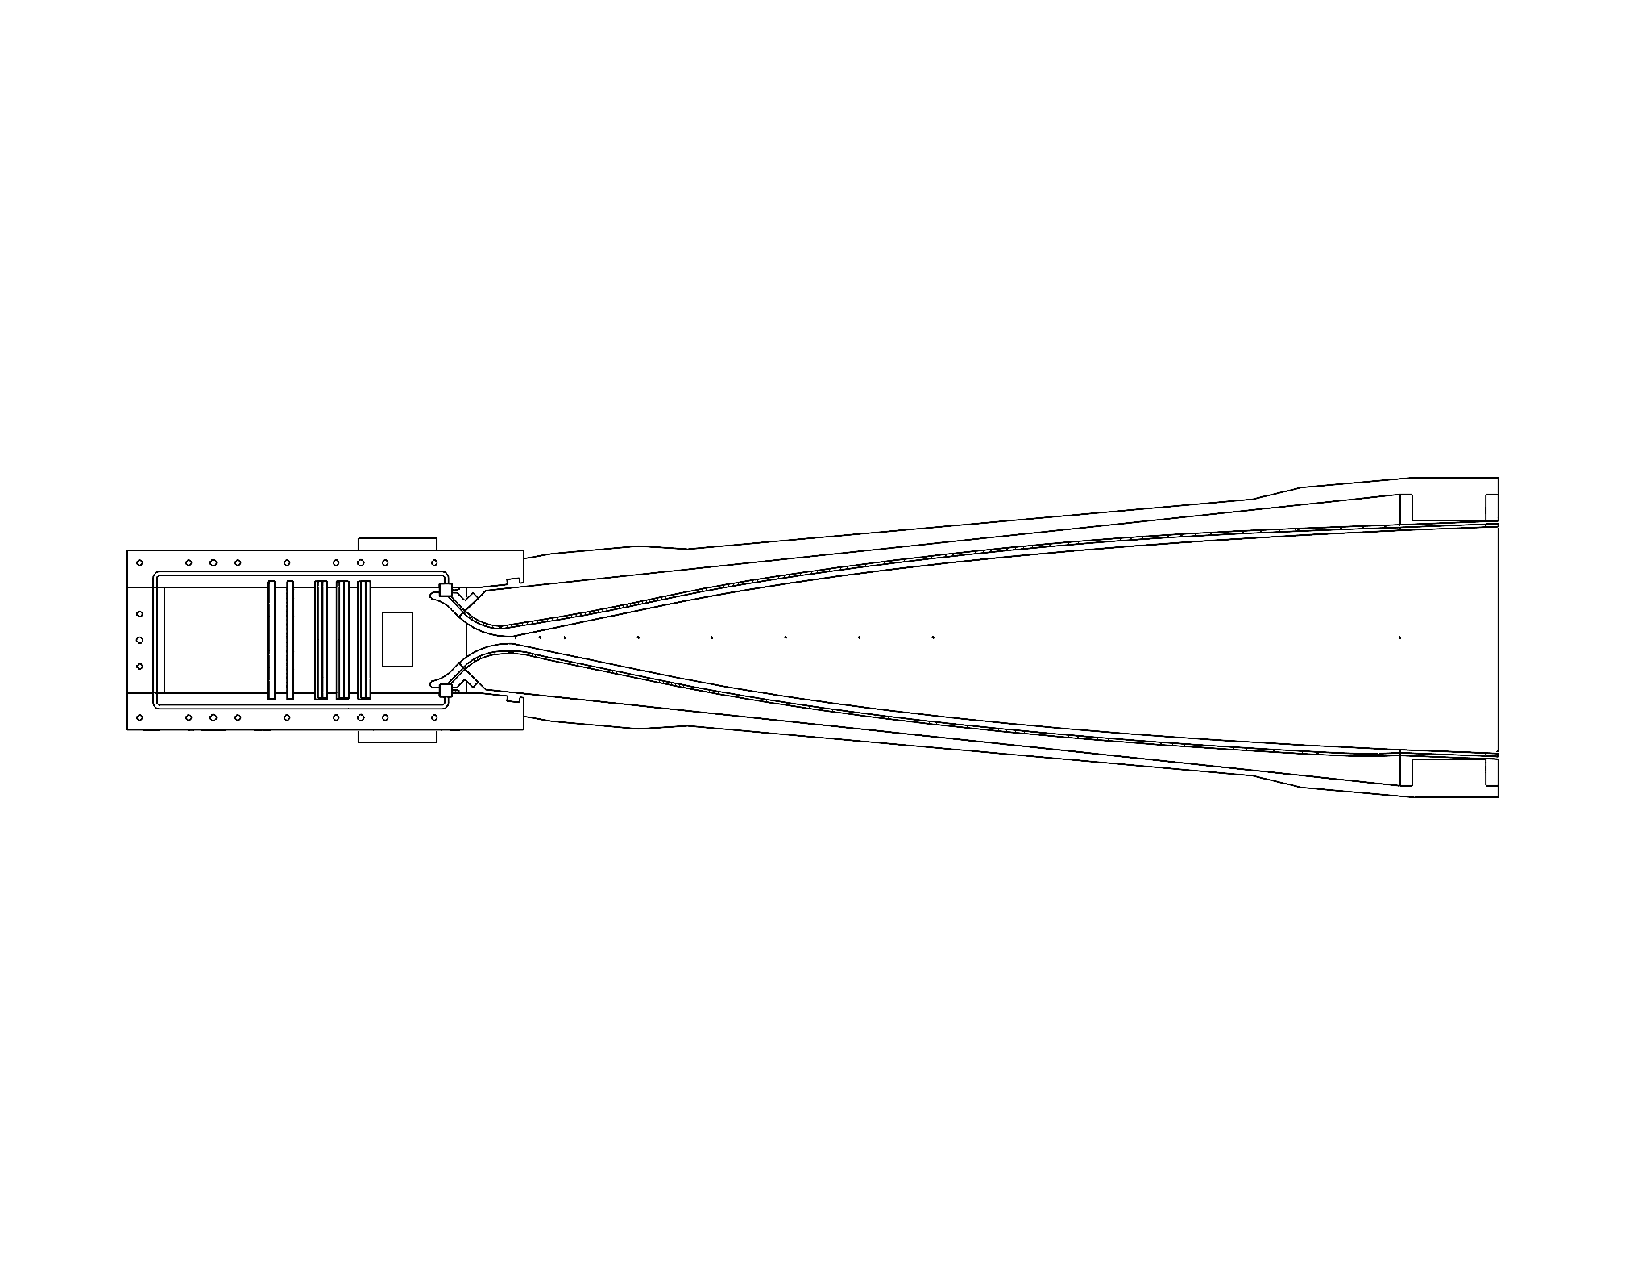
\includegraphics[trim={40 220 40 220},clip,width=6in]{ace-nozzle.pdf}
    \caption{ACE nozzle and settling chamber}
    \label{fig:ace-nozzle}
\end{figure}

The original motivation for the redesign was to remanufacture the nozzle to remedy the premature laminar-to-turbulent transition, which is discussed in the next section. However, as the redesign progressed, it became apparent that this was the best opportunity to completely redesign the nozzle and settling chamber to enable active control. This progression and the redesign process is detailed throughout this chapter.

\subsection{ACE Turbulent Transition}

ACE performance data \cite{aceturb,mai-dis,neel-dis,leidy-dis} shows that below a unit Reynolds number of $Re'$ = $\frac{\rho U}{\mu} \approx 3 \times 10^6/\mathrm{m}$ the RMS pressure fluctuations in the test section are less than 1\%, and that above this unit Reynolds number the pressure fluctuation levels significantly increase. It was desired to increase the unit Reynolds number at which laminar flow can be maintained, so the mechanism causing laminar-to-turbulent transition of the nozzle boundary layers had to be determined. The hypothesis and supporting data regarding the pressure fluctuation levels increase and how it might be delayed to higher unit Reynolds numbers is summarized below.

Five primary suspects for transition were identified:

\begin{enumerate}
    \item A known manufacturing surface discontinuity at the nozzle throat
    \item Sidewall mushroom vortices
    \item Görtler vortices
    \item Freestream turbulence in the incoming flow and/or upstream boundary layer
    \item Wall roughness or waviness
\end{enumerate}

\textcolor{red}{How did lip occur, how big, and where?} The throat discontinuity (1) is the result of a decimal truncation error when connecting the subsonic curve to the supersonic MOC contour in Solidworks. The resulting discontinuity can be seen in Figure \ref{fig:ace-throat}, and it has a height of around 0.0003 inches. 

\begin{figure}[ht]
    \centering
    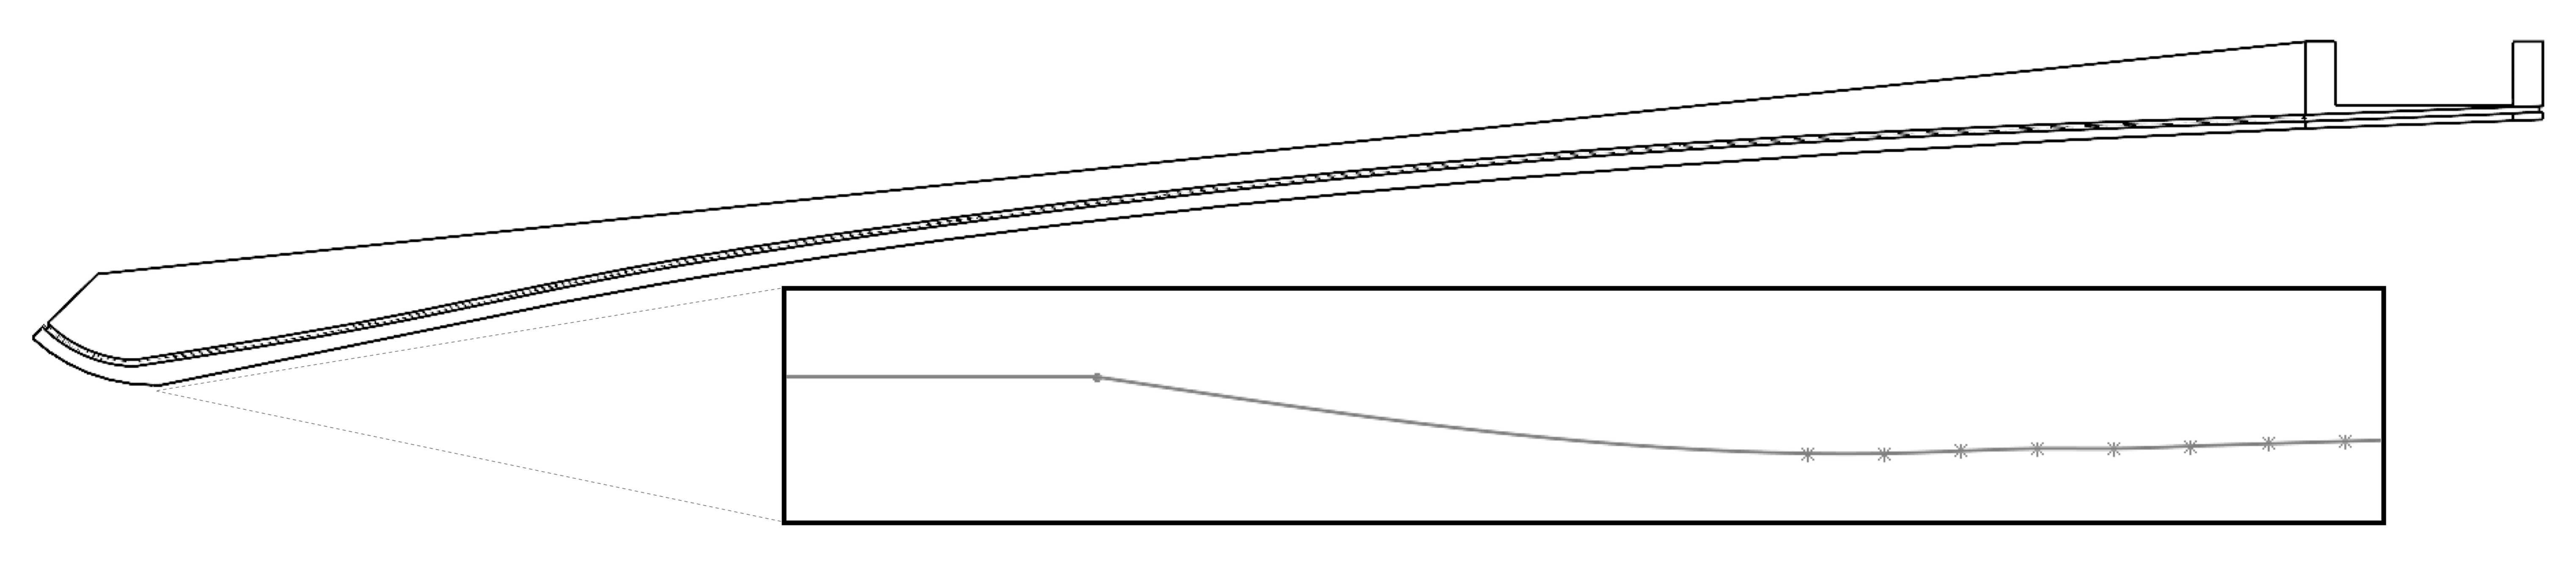
\includegraphics[width=6in]{ace-throat}
    \caption{ACE throat discontinuity}
    \label{fig:ace-throat}
\end{figure}


The sections below evaluate each of these possibilities and support the conclusion that the throat discontinuity is the most likely reason for the increased pressure fluctuations above $Re' \approx 3 \times 10^6/\mathrm{m}$. This conclusion is supported by pitot surveys, method-of-characteristics line tracing, and CFD simulations. Sidewall mushroom vortices (2) and Görtler vortices (3) would lead to transition too far downstream from the throat to be responsible for the pressure fluctuation levels increase. Incoming freestream turbulence (4) and wall surface quality (5) are potential causes of poor flow quality in all supersonic tunnels and are included for completeness. The specific mechanism by which these would cause transition is not known. While item 4 and 5 are not the primary suspects for the pressure fluctuation levels increase, improving these conditions will be addressed in the redesign intended to extend laminar flow to higher unit Reynolds numbers.

\subsubsection*{ACE Nozzle Noise Surveys}

Three recent pitot surveys have been conducted in the ACE tunnel. The first by Mai in 2014 \cite{mai-dis} revealed transition occurring around $Re' \approx 3 \times 10^6/\mathrm{m}$, as shown in Figure \ref{fig:mai-survey}. The same result was found by Neel in 2019 \cite{neel-dis} shown in Figure \ref{fig:neel-survey} that transition occurs at this $Re'$ value at a location 6 inches upstream of the nozzle exit. A final pitot survey in ACE by Wirth in 2022 (unpublished) was conducted to determine whether the pressure fluctuation levels increase occurred at different $Re'$ values at positions farther upstream in the nozzle. He found pressure fluctuation levels increase at $Re' \approx 3 \times 10^6/\mathrm{m}$ at a measurement location 17 inches upstream of the nozzle exit. His results in Figure \ref{fig:wirth-survey} align perfectly with Mai's and Neel's data and clearly establish that the Reynolds number at which pressure fluctuation levels increase is the same at all locations in the nozzle. This suggests that transition is not moving upstream through the nozzle as Reynolds number is increased.

\begin{figure}[ht!]
    \centering
    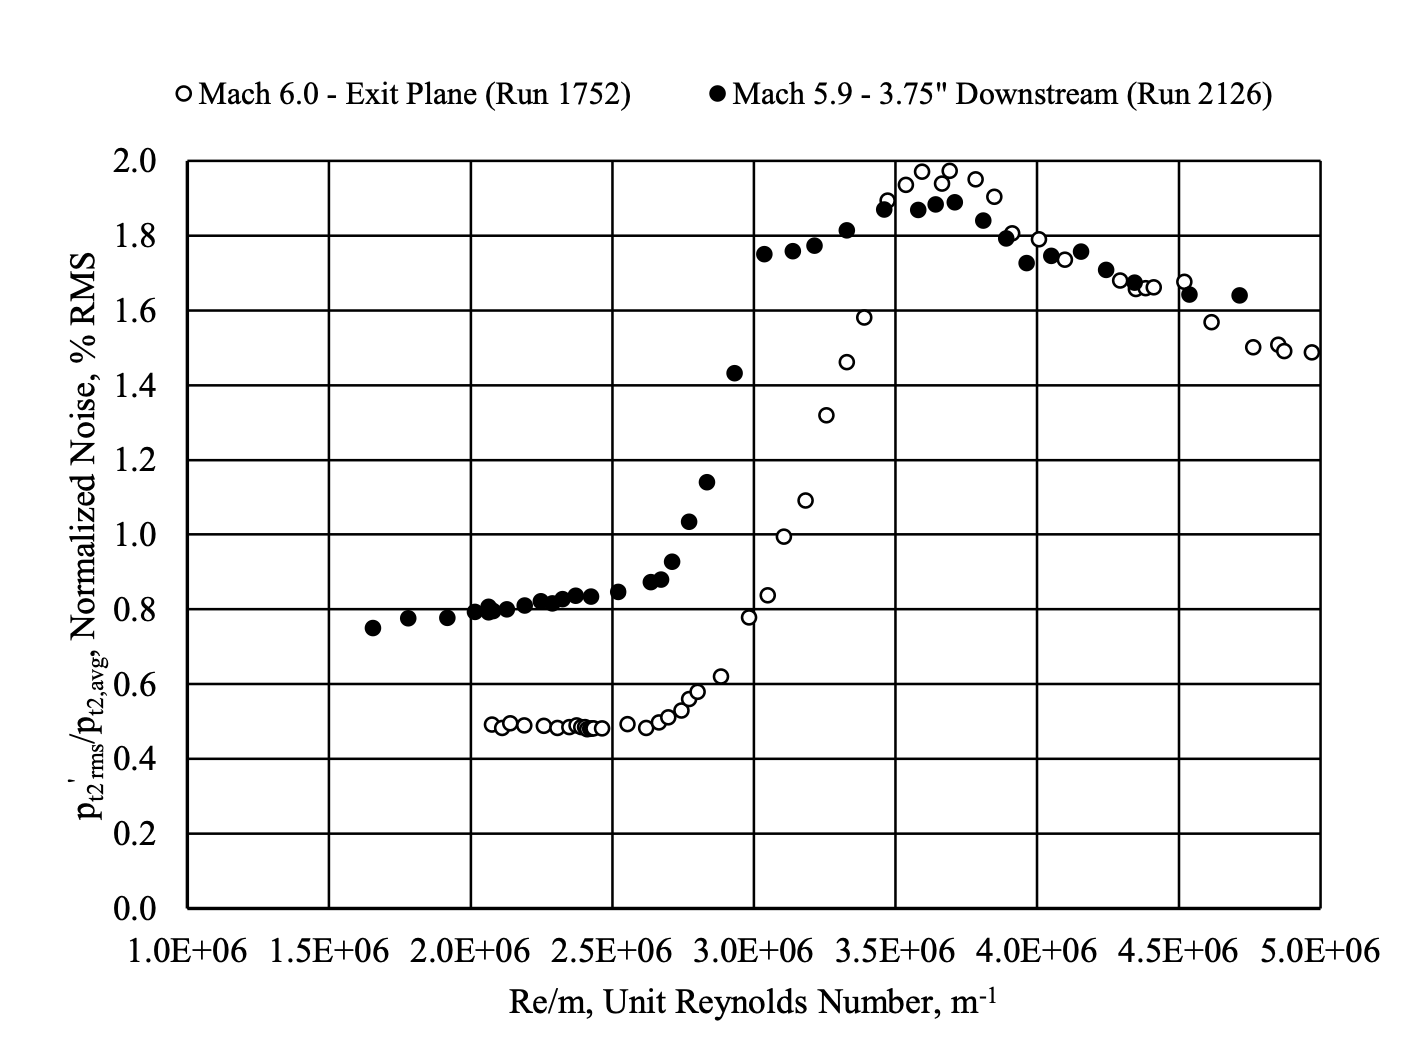
\includegraphics[width=6in]{mai-survey}
    \caption[ACE freestream pressure fluctuations in the nozzle exit plane as measured in 2014]{ACE freestream pressure fluctuations in the nozzle exit plane as measured in 2014 \cite{mai-dis}}
    \label{fig:mai-survey}
\end{figure}

\begin{figure}[ht!]
    \centering
    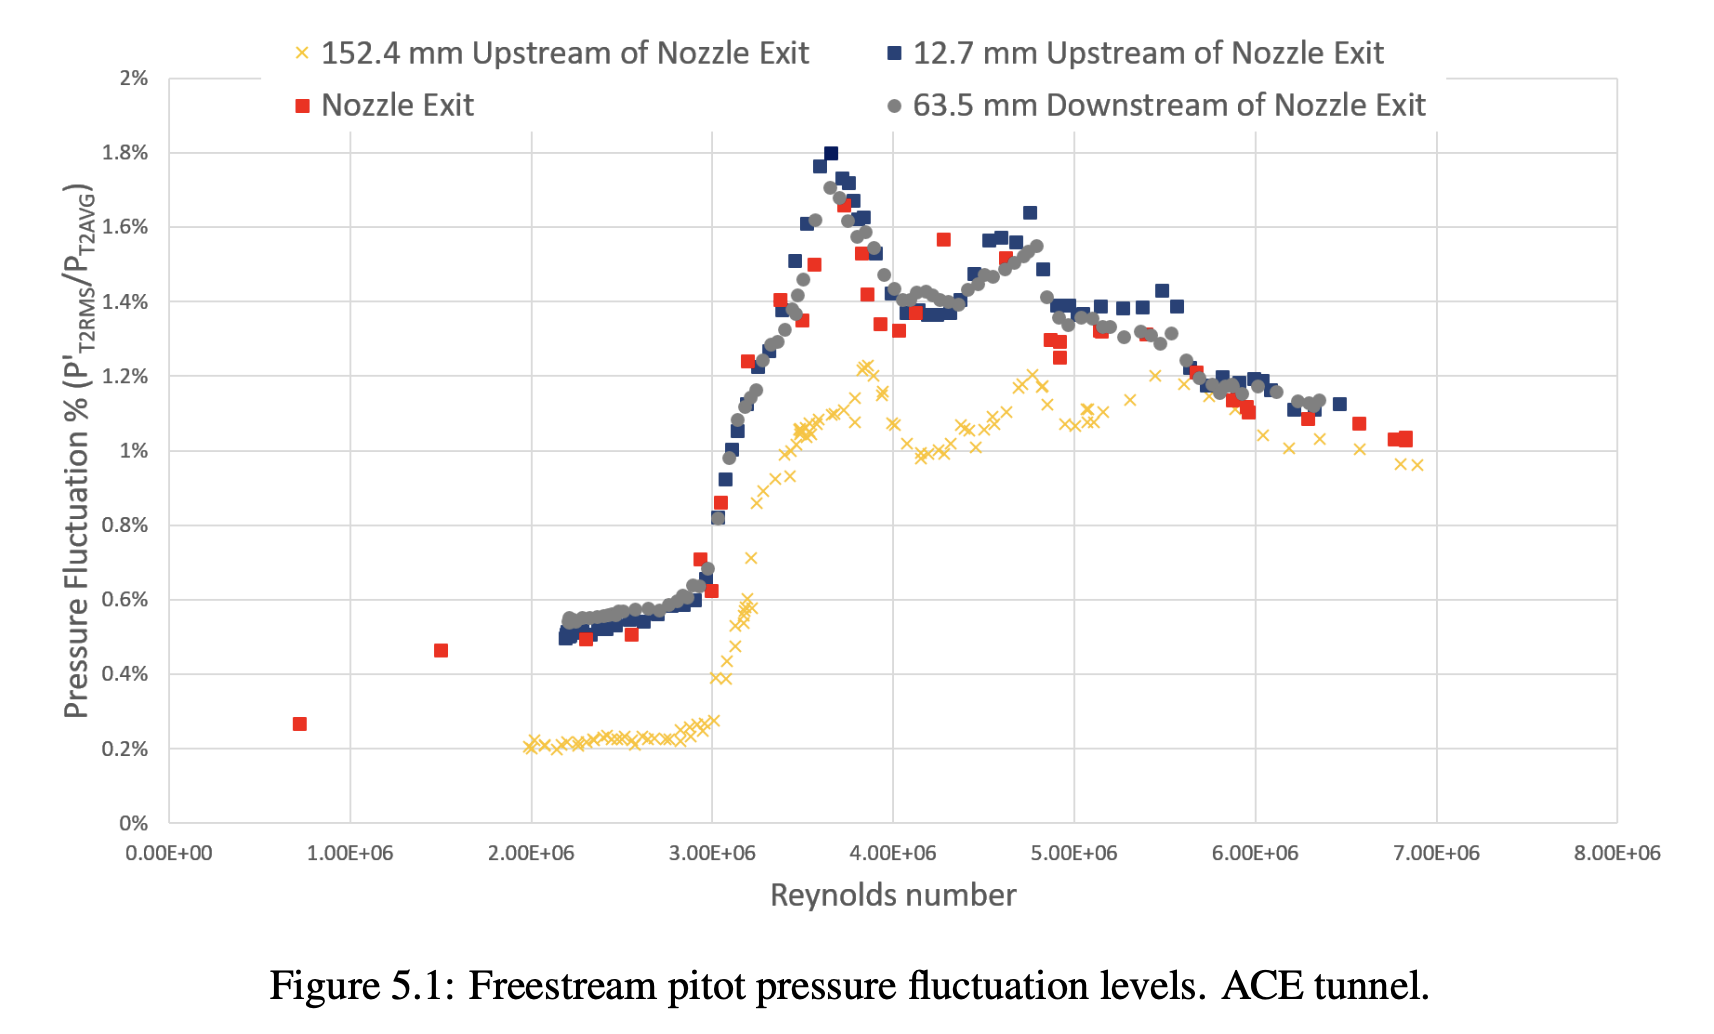
\includegraphics[width=6in]{neel-survey}
    \caption[ACE freestream pressure fluctuations at various locations as measured ii 2019]{ACE freestream pressure fluctuations at various locations as measured in 2019 \cite{neel-dis}}
    \label{fig:neel-survey}
\end{figure}

\begin{figure}[ht!]
    \centering
    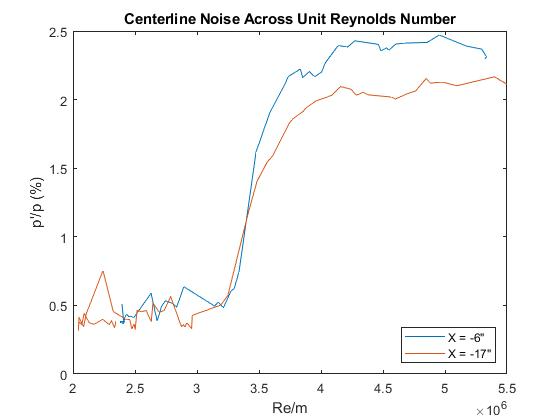
\includegraphics[width=6in]{wirth-survey}
    \caption{ACE freestream pressure fluctuations at 6 inches and 17 inches upstream of nozzle exit as measured in 2022}
    \label{fig:wirth-survey}
\end{figure}

\subsubsection*{Suspect Mechanism Conclusions}

The pressure fluctuation levels revealed the $Re'$ value at which transition occurs but not the transition mechanism. The two mechanisms that were extensively investigated at the start of this work were sidewall mushroom vortices and Görtler vortices. Sidewall mushroom vortices arise from the pressure distribution in the low momentum flow in the sidewall boundary layers. The flow at the centerline expands to the test section pressure ahead of the top and bottom curved walls. The flow at the top and bottom lags behind the centerline flow with a higher pressure to create a vertical pressure gradient that introduces a secondary vertical flow in the sidewall boundary layers that flows from the corners to the centerline \cite{sabnis}. CFD simulations by Kocian (unpublished) show the sidewall mushroom vortices beginning to form approximately 24 inches upstream of the nozzle exit shown in Figures \ref{fig:mushrooms} and \ref{fig:vertical-vel}. 
\begin{figure}[ht!]
    \centering
    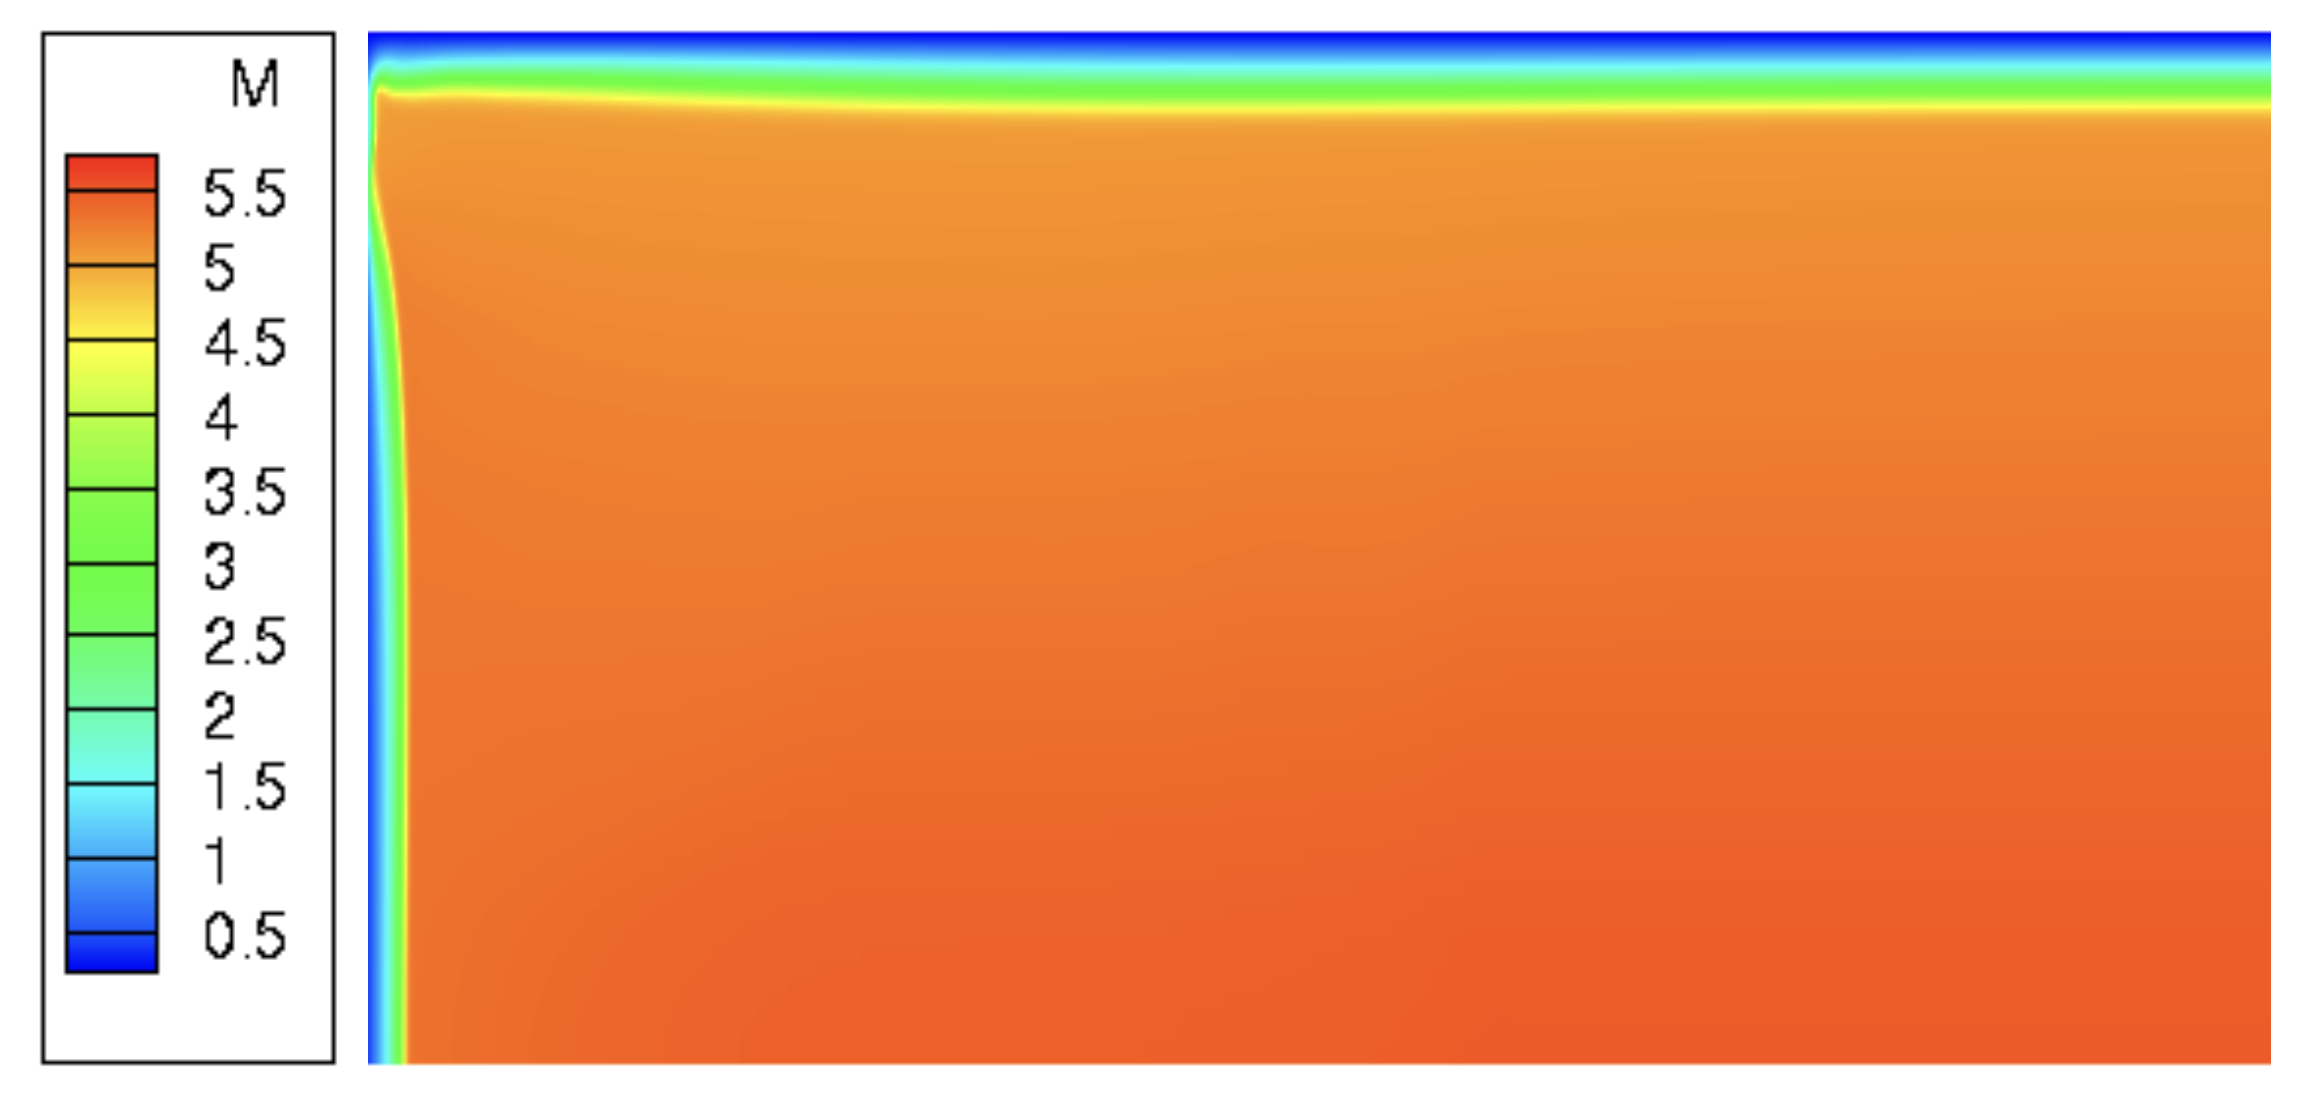
\includegraphics[width=5in]{mush24}
    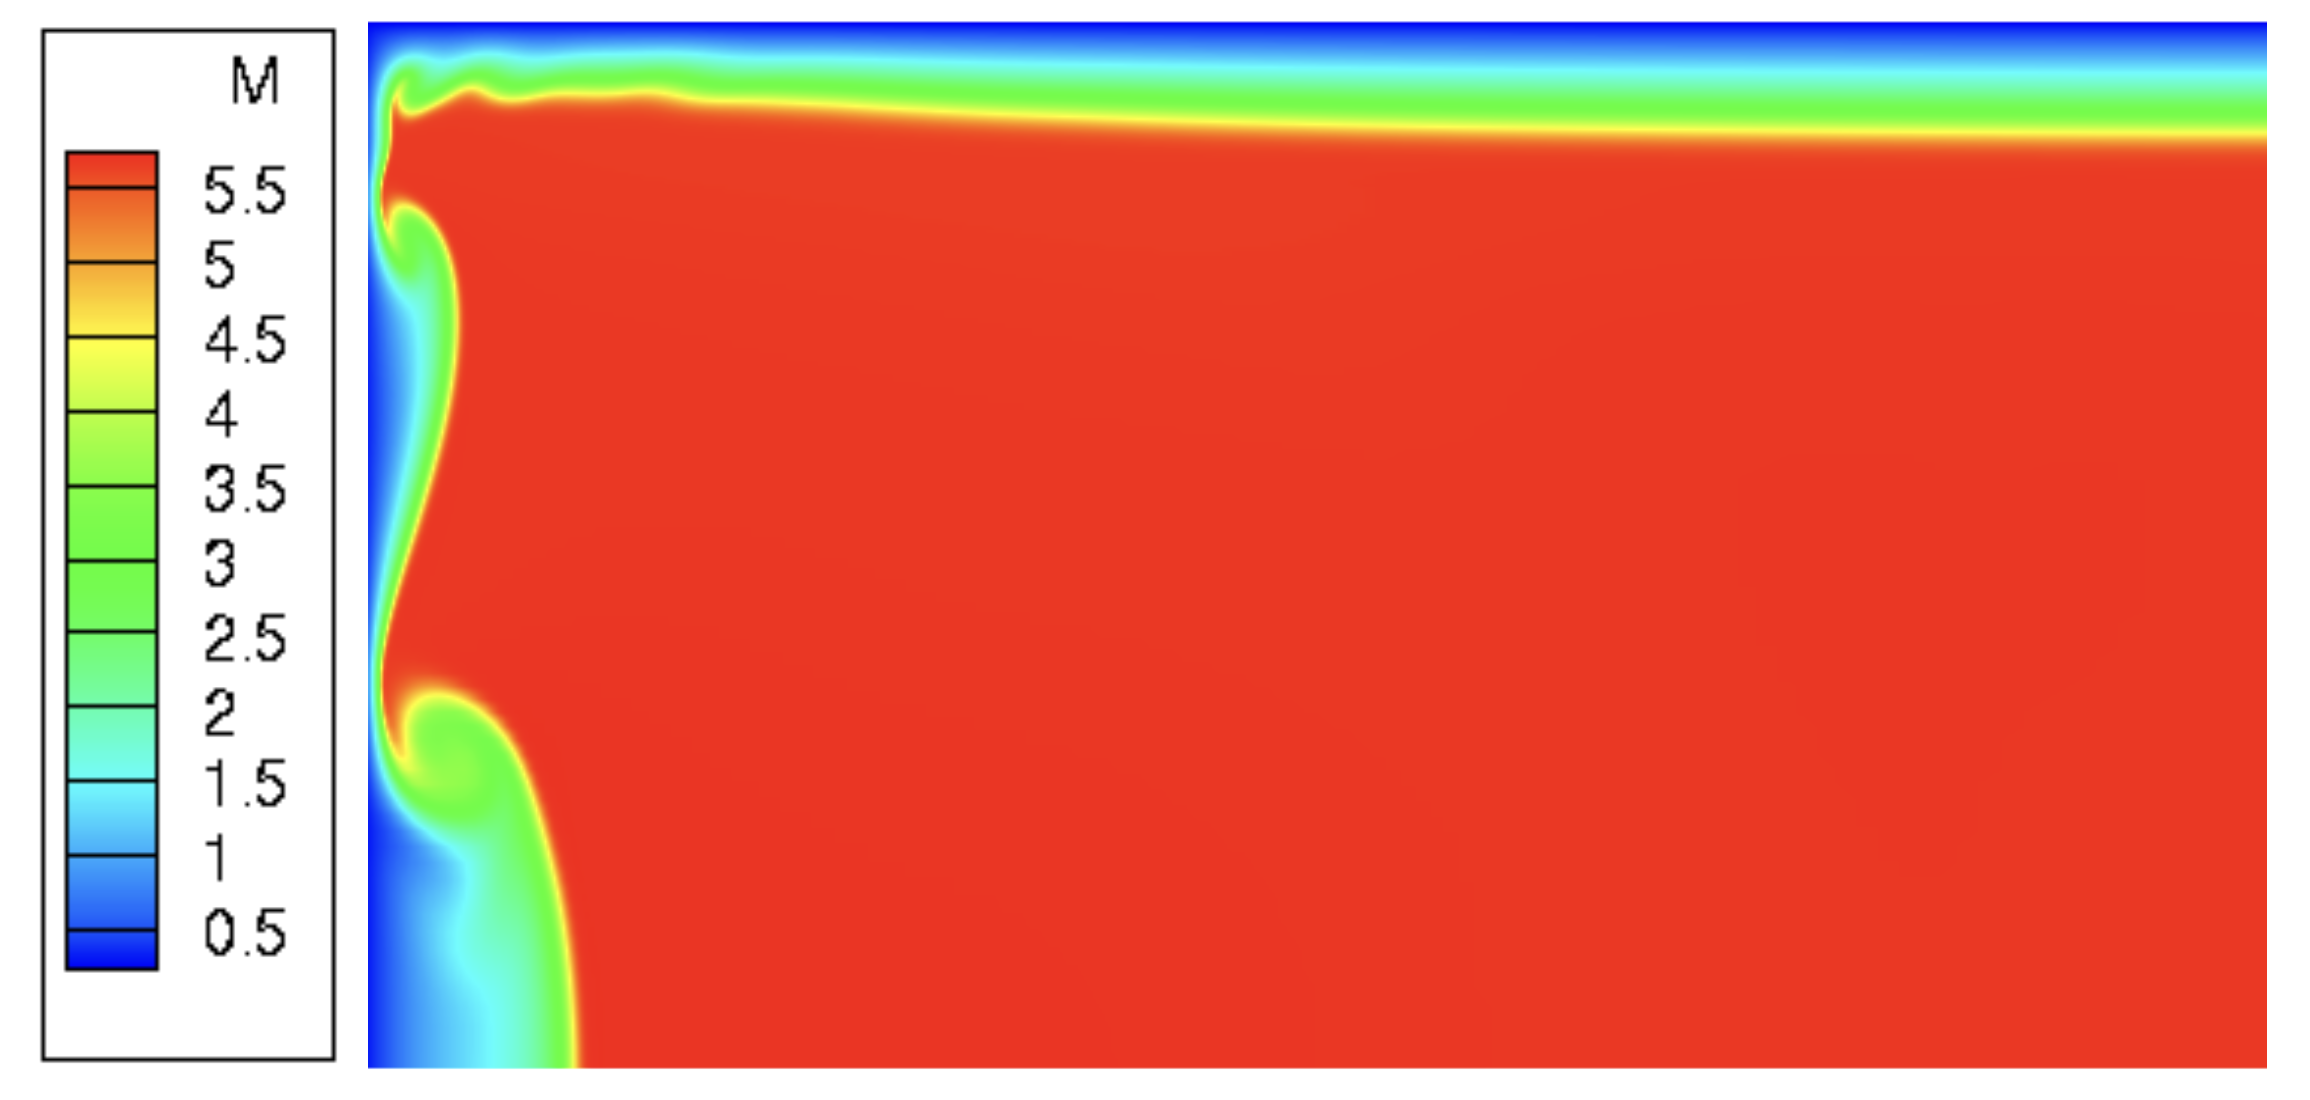
\includegraphics[width=5in]{mush0}
    \caption{Mushroom vortex formation at sidewalls}
    \label{fig:mushrooms}
\end{figure}

\begin{figure}[ht!]
    \centering
    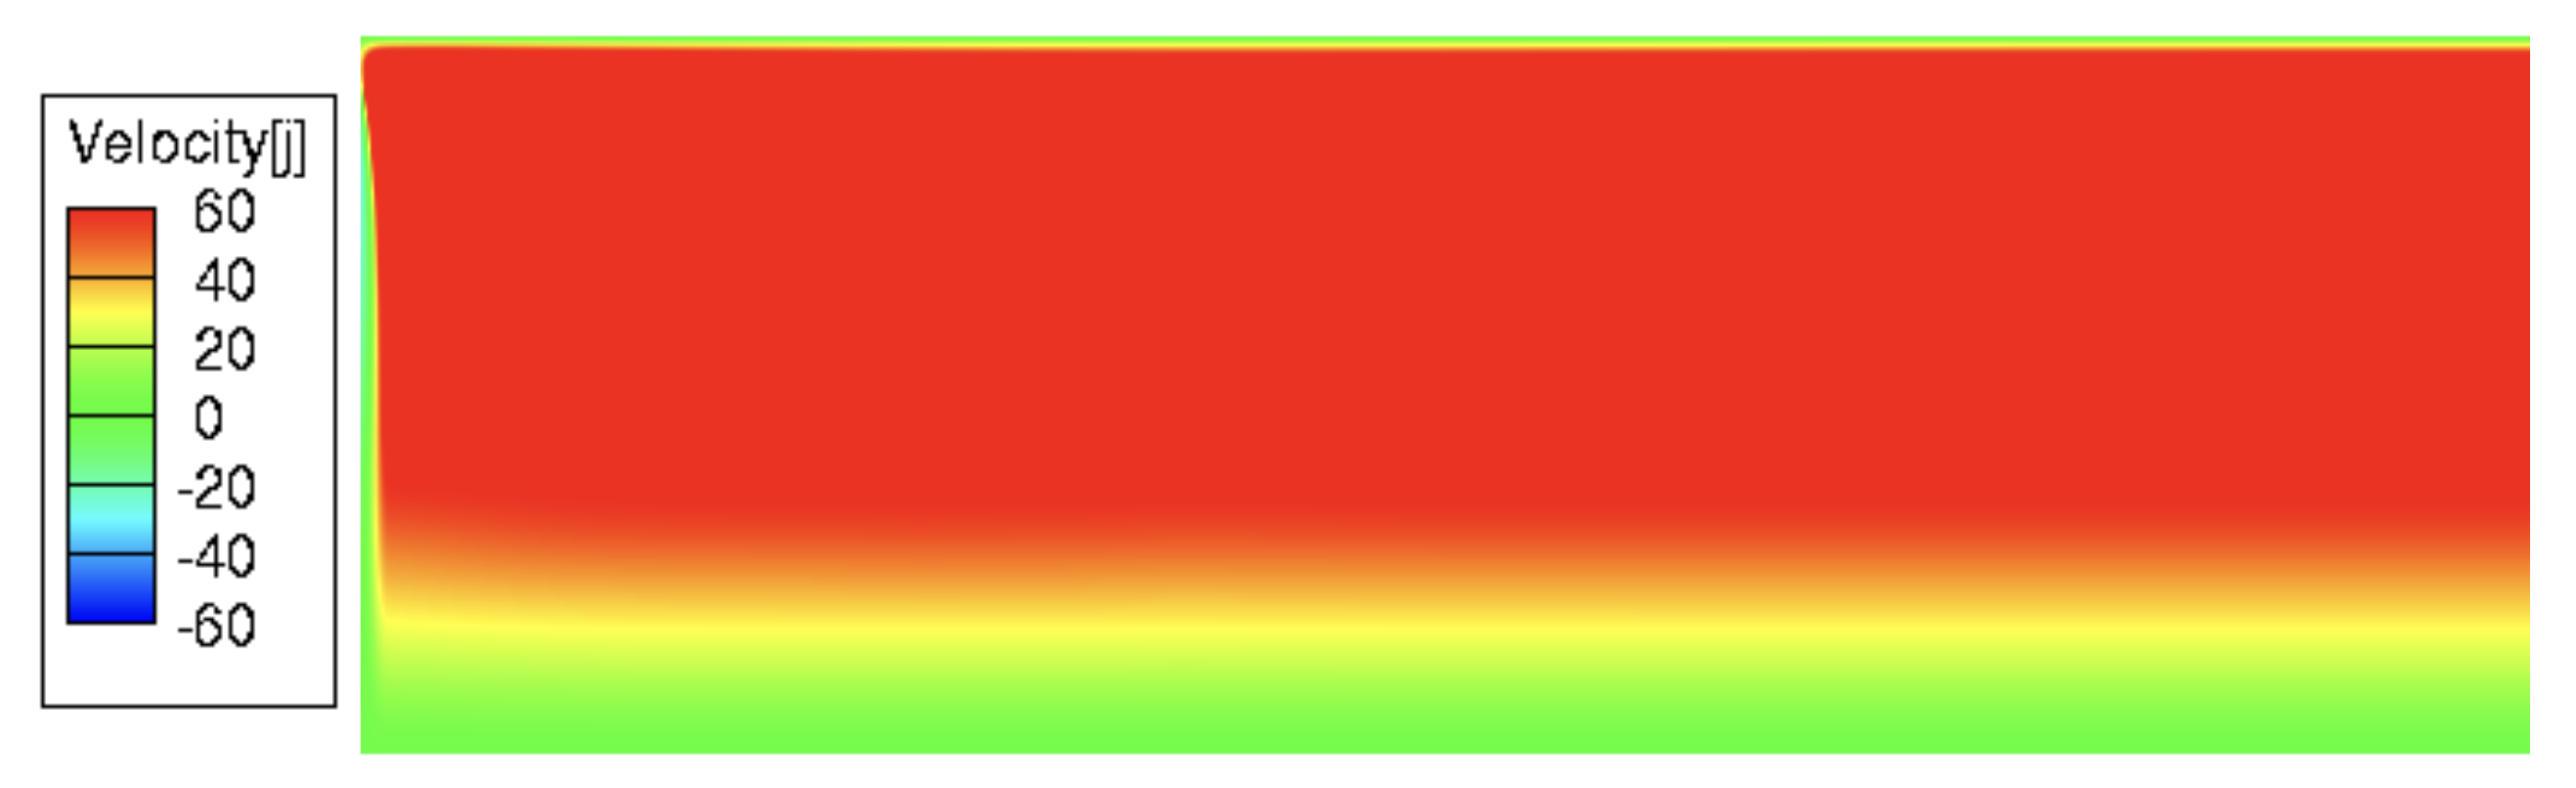
\includegraphics[width=5in]{vertical28}
    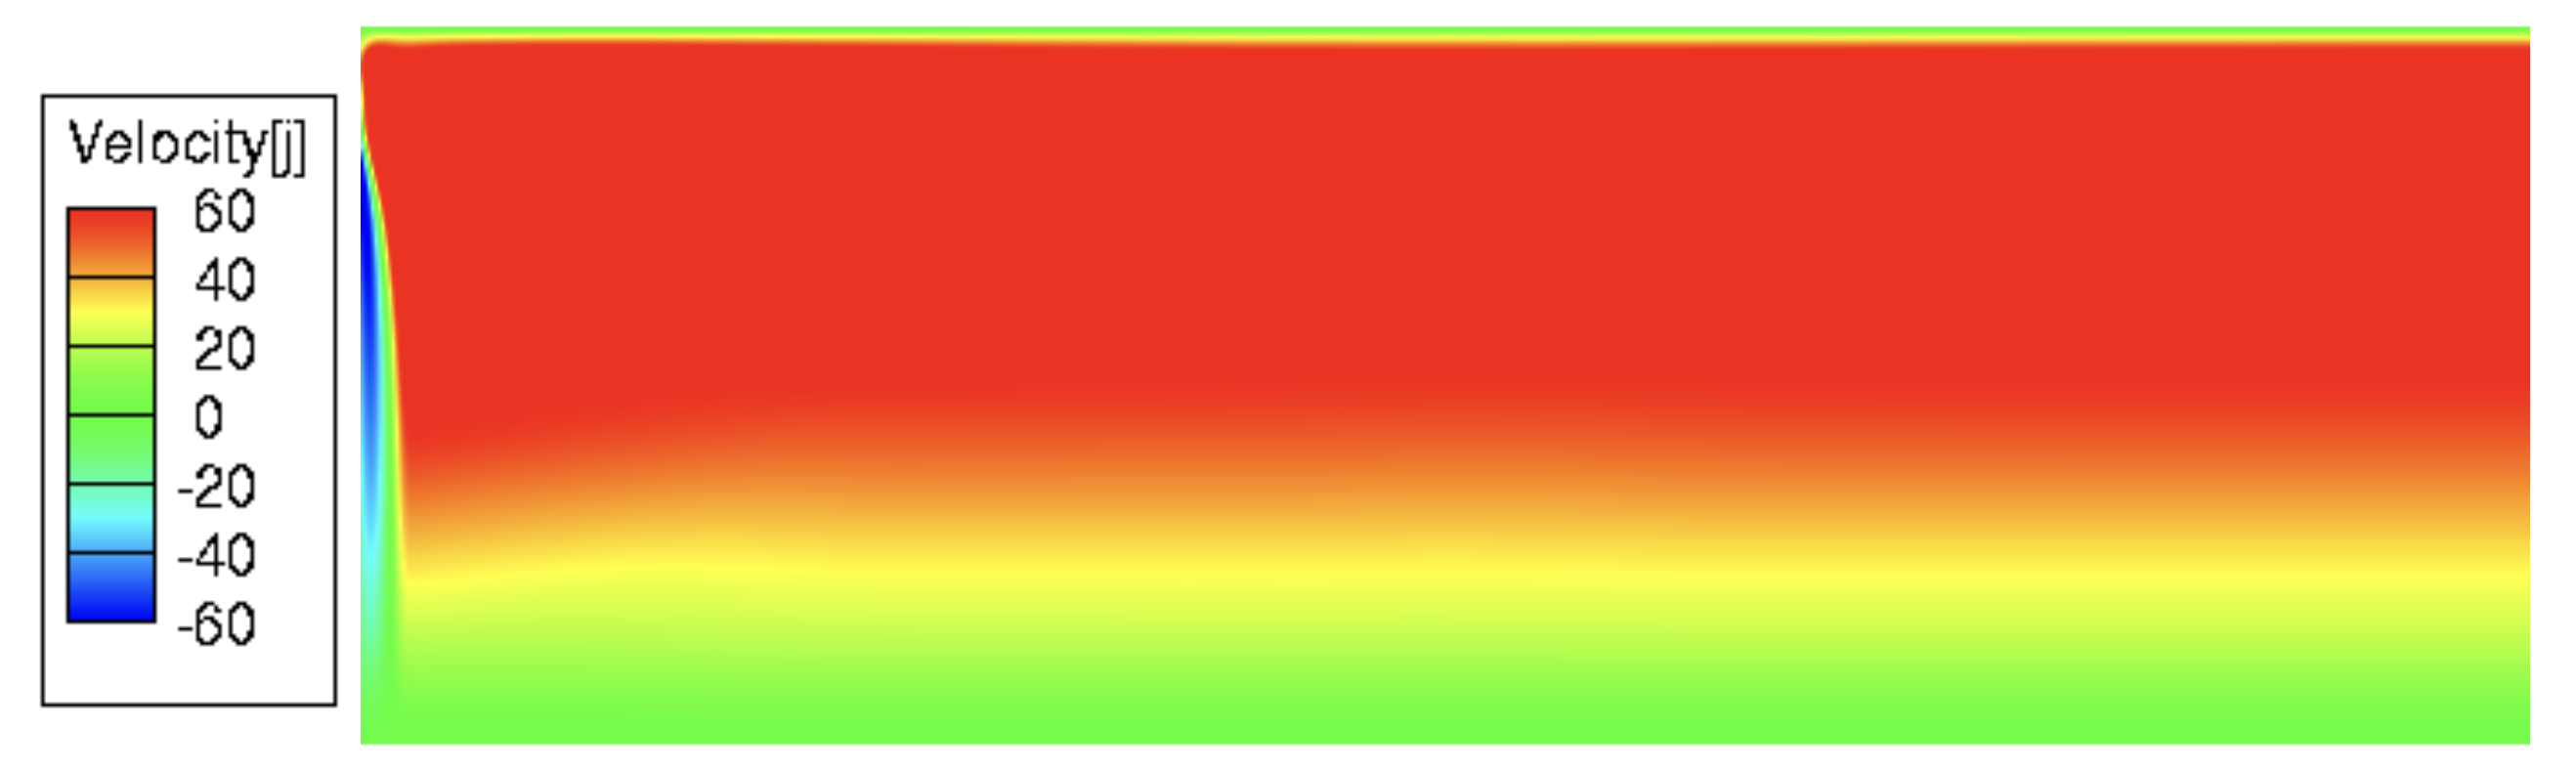
\includegraphics[width=5in]{vertical24}
    \caption{Vertical velocity}
    \label{fig:vertical-vel}
\end{figure}

Görtler vortices are counter-rotating streamwise vortices that occur in boundary layers on concave surfaces \cite{saric}. To estimate where these may lead to transition, a CFD basic state simulation and N-factor analysis was performed by Kocian in 2022 (unpublished). The results, shown in Figures \ref{} and \ref{}, indicate that Görtler vortices could induce transition around 8 inches from the nozzle throat. \textcolor{red}{Elaborate on findings with plots}

\begin{figure}[ht]
    \centering
    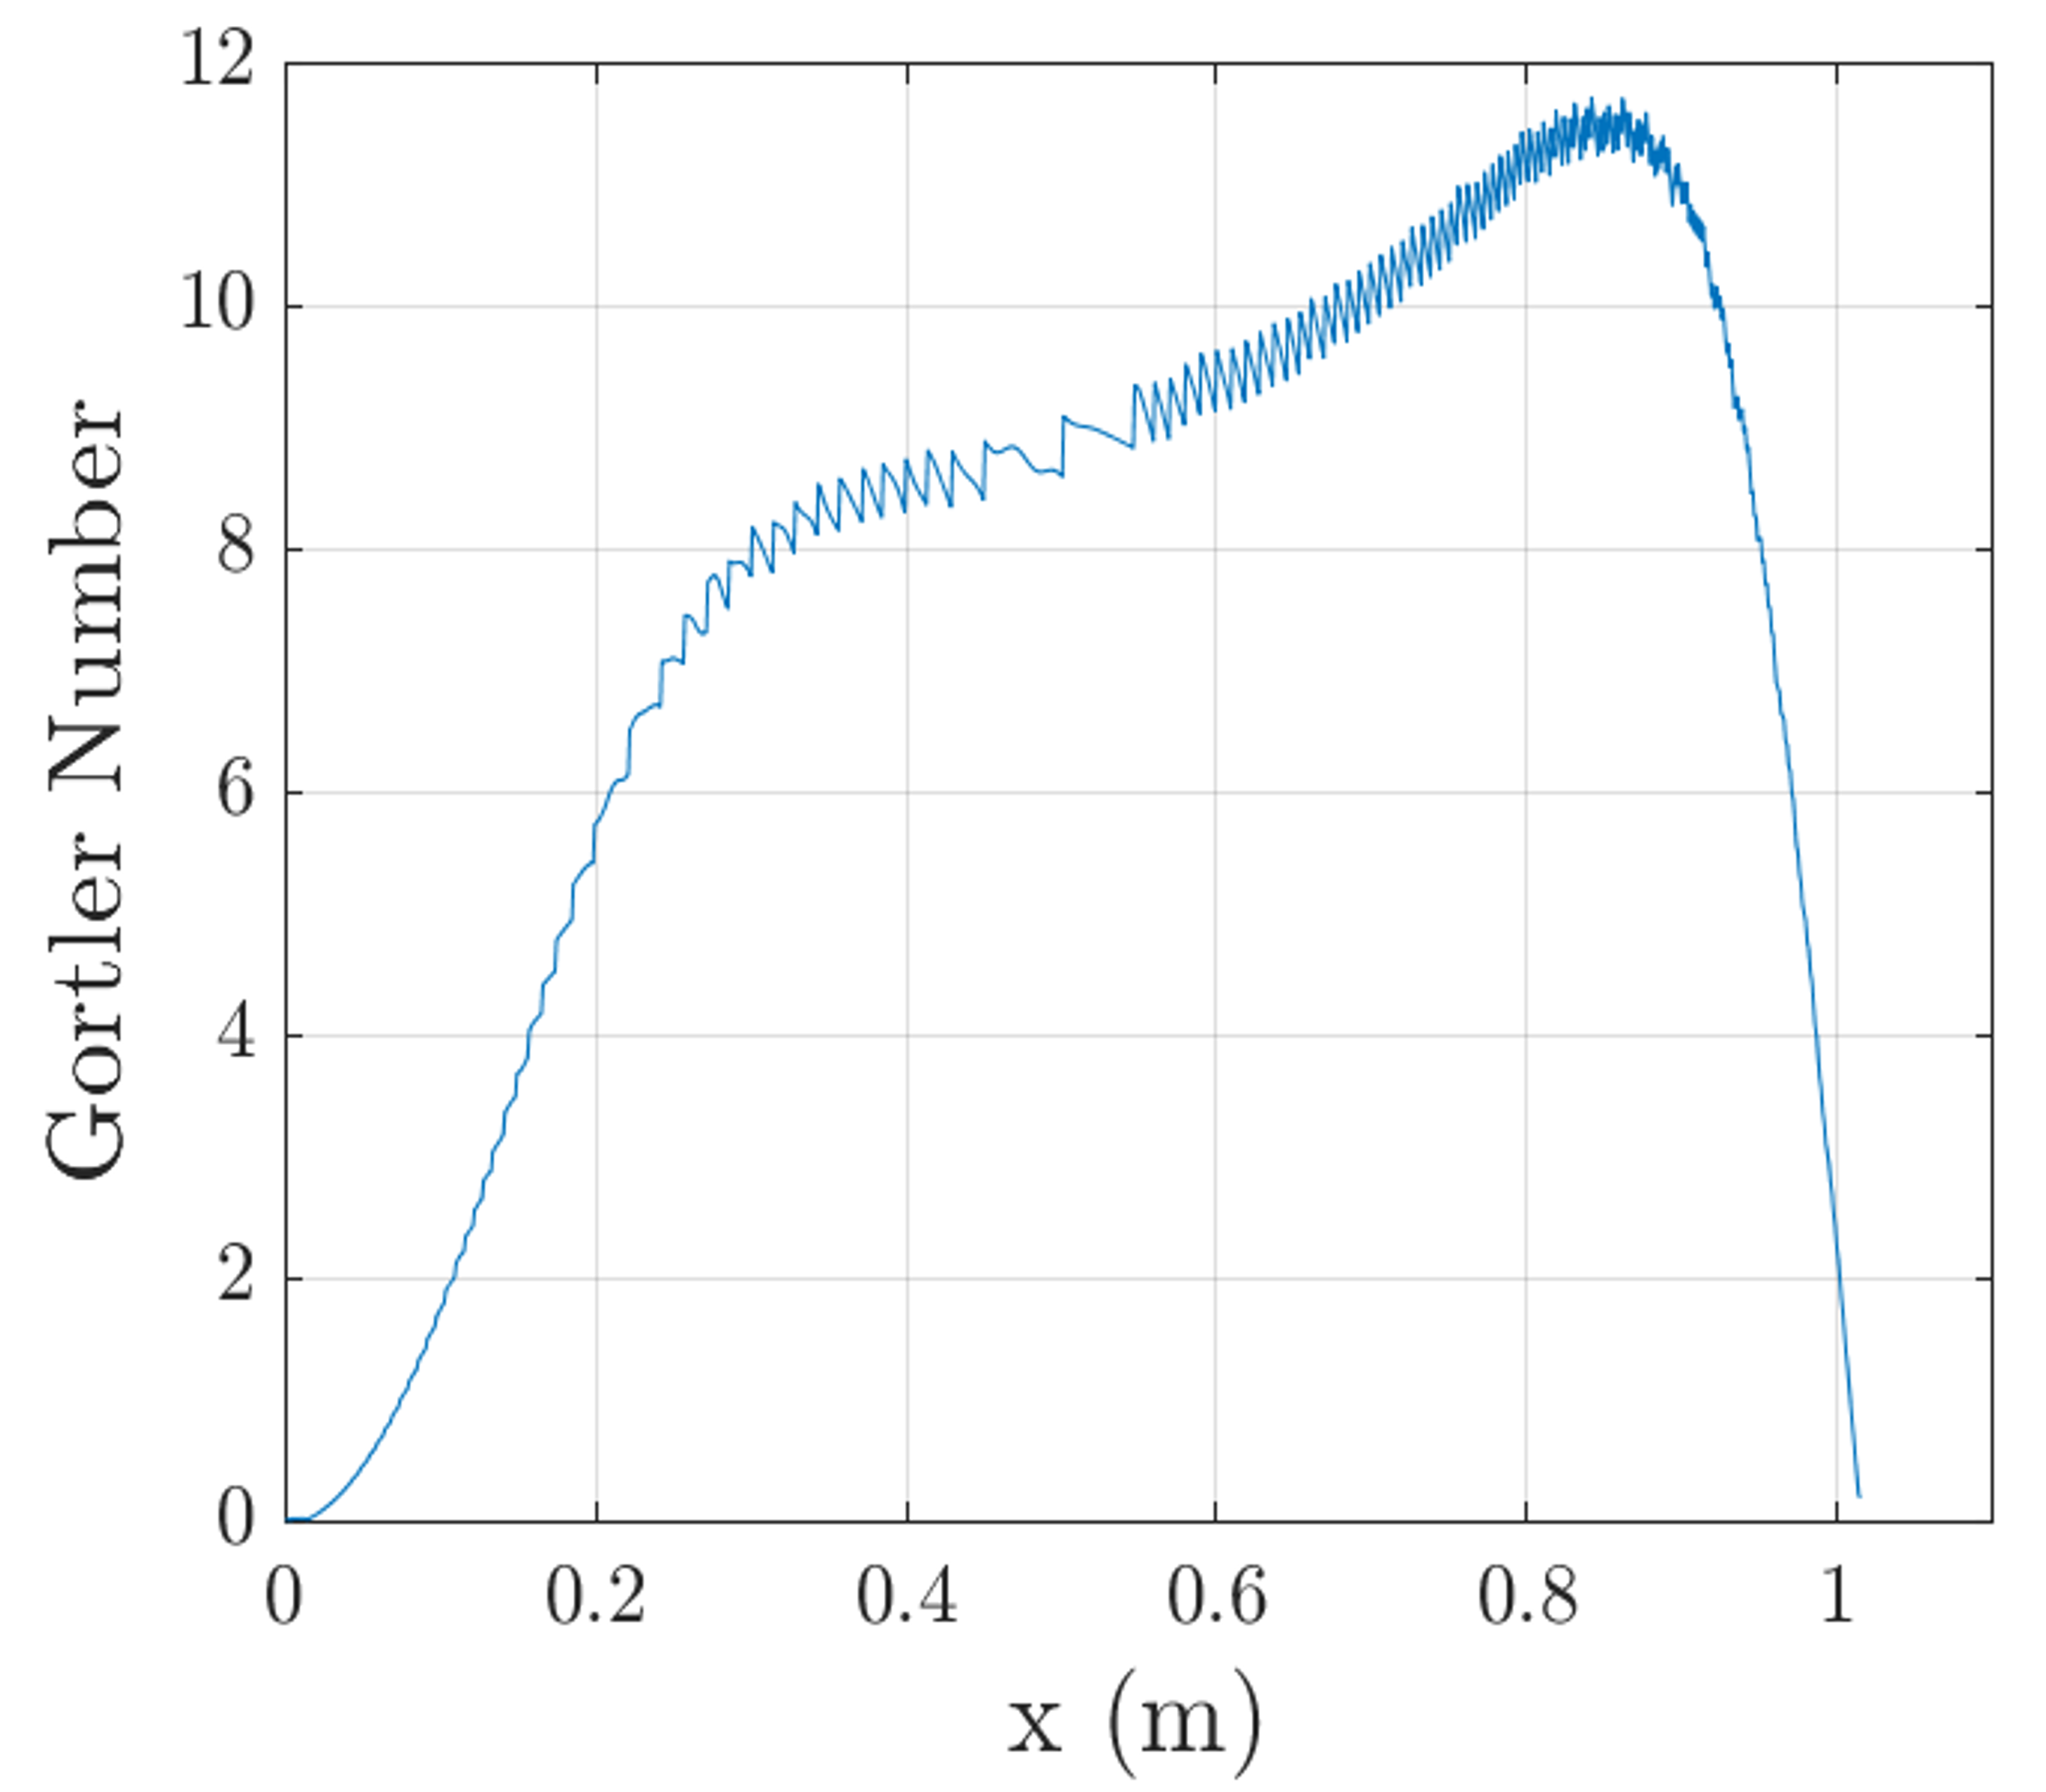
\includegraphics[width=5in]{gortler}
    \caption{Görtler number from ACE nozzle CFD}
    \label{fig:gortler}
\end{figure}

\begin{figure}[ht]
    \centering
    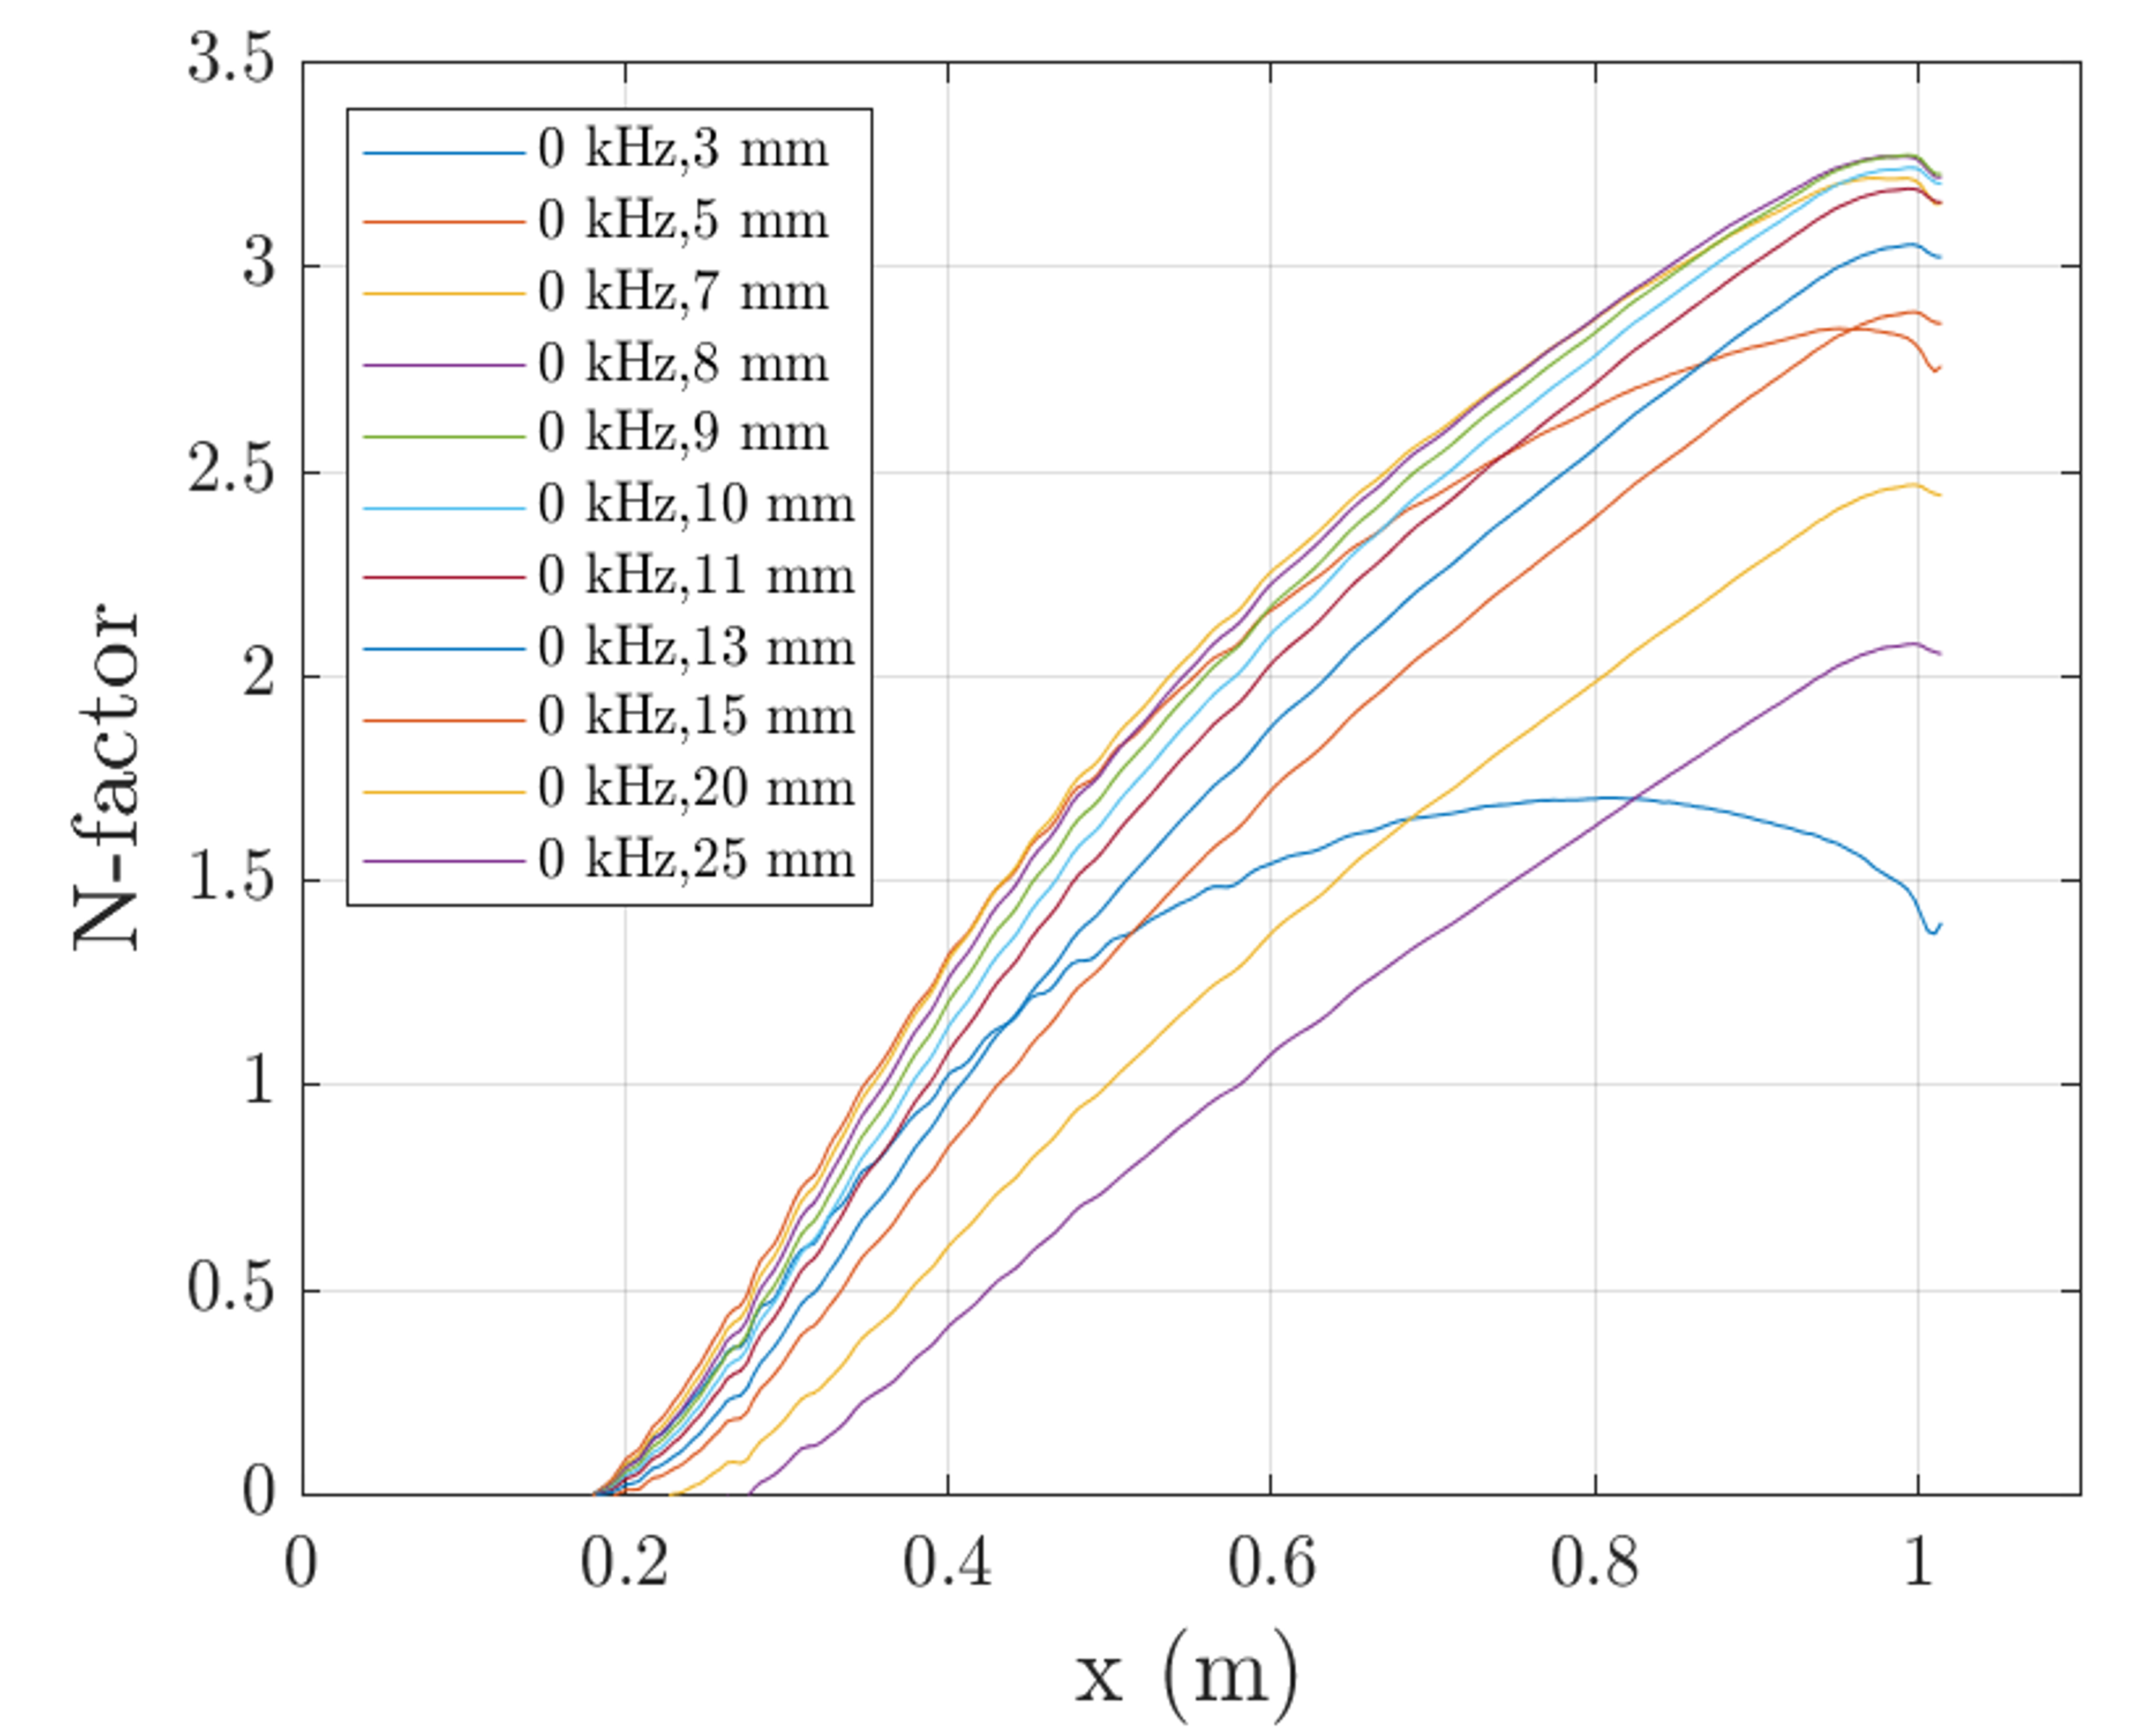
\includegraphics[width=5in]{n-factor}
    \caption{N-factors for Görtler number in ACE nozzle}
    \label{fig:n-factor}
\end{figure}

\textcolor{red}{Starting here discuss characteristic tracing how plus results and conclusion re: noise, mushroom, Görtler}

The origin of the noise measured farthest upstream of the nozzle exit was determined by tracing characteristic lines from the measurement location at the centerline upstream to the wall. Both the side view and top view of this can be seen in Figure \ref{fig:machlines}. \textcolor{red}{Expand on this with more info. How did you do it? What conclusions did you draw?}

\textcolor{red}{Tracing the characteristics from 17 inches upstream of the nozzle exit, Figure \ref{fig:machlines} shows the origin to be upstream of the throat where sidewall mushroom vortices are not relevant.}

\textcolor{red}{However, tracing the characteristics from 17 inches upstream of the nozzle exit, Figure \ref{fig:machlines} shows the measured noise originates at the end of the straight section of the nozzle where Görtler is not relevant.}

\begin{figure}[ht!]
    \centering
    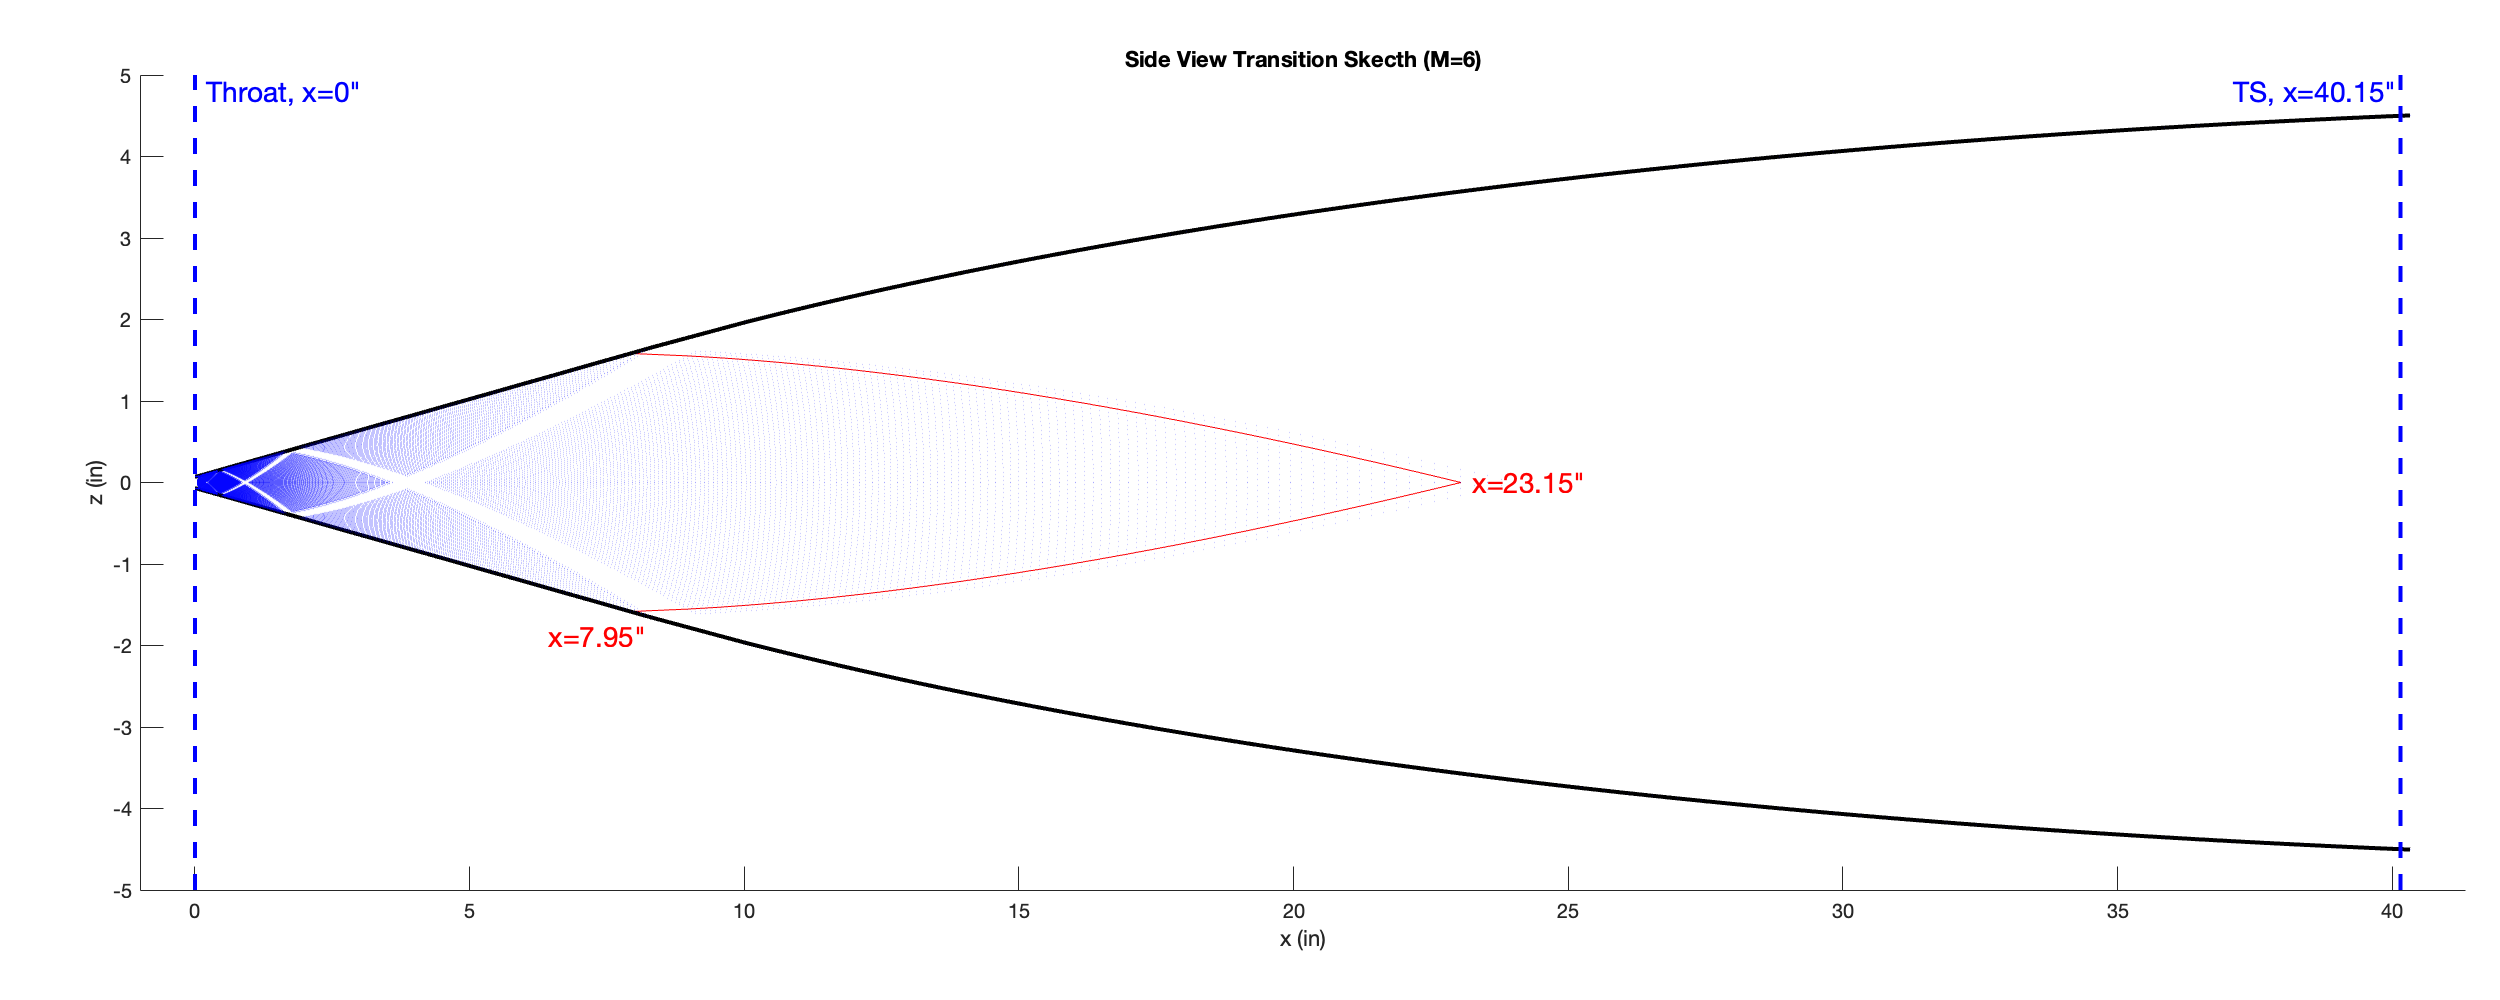
\includegraphics[width=6.5in]{side17}
    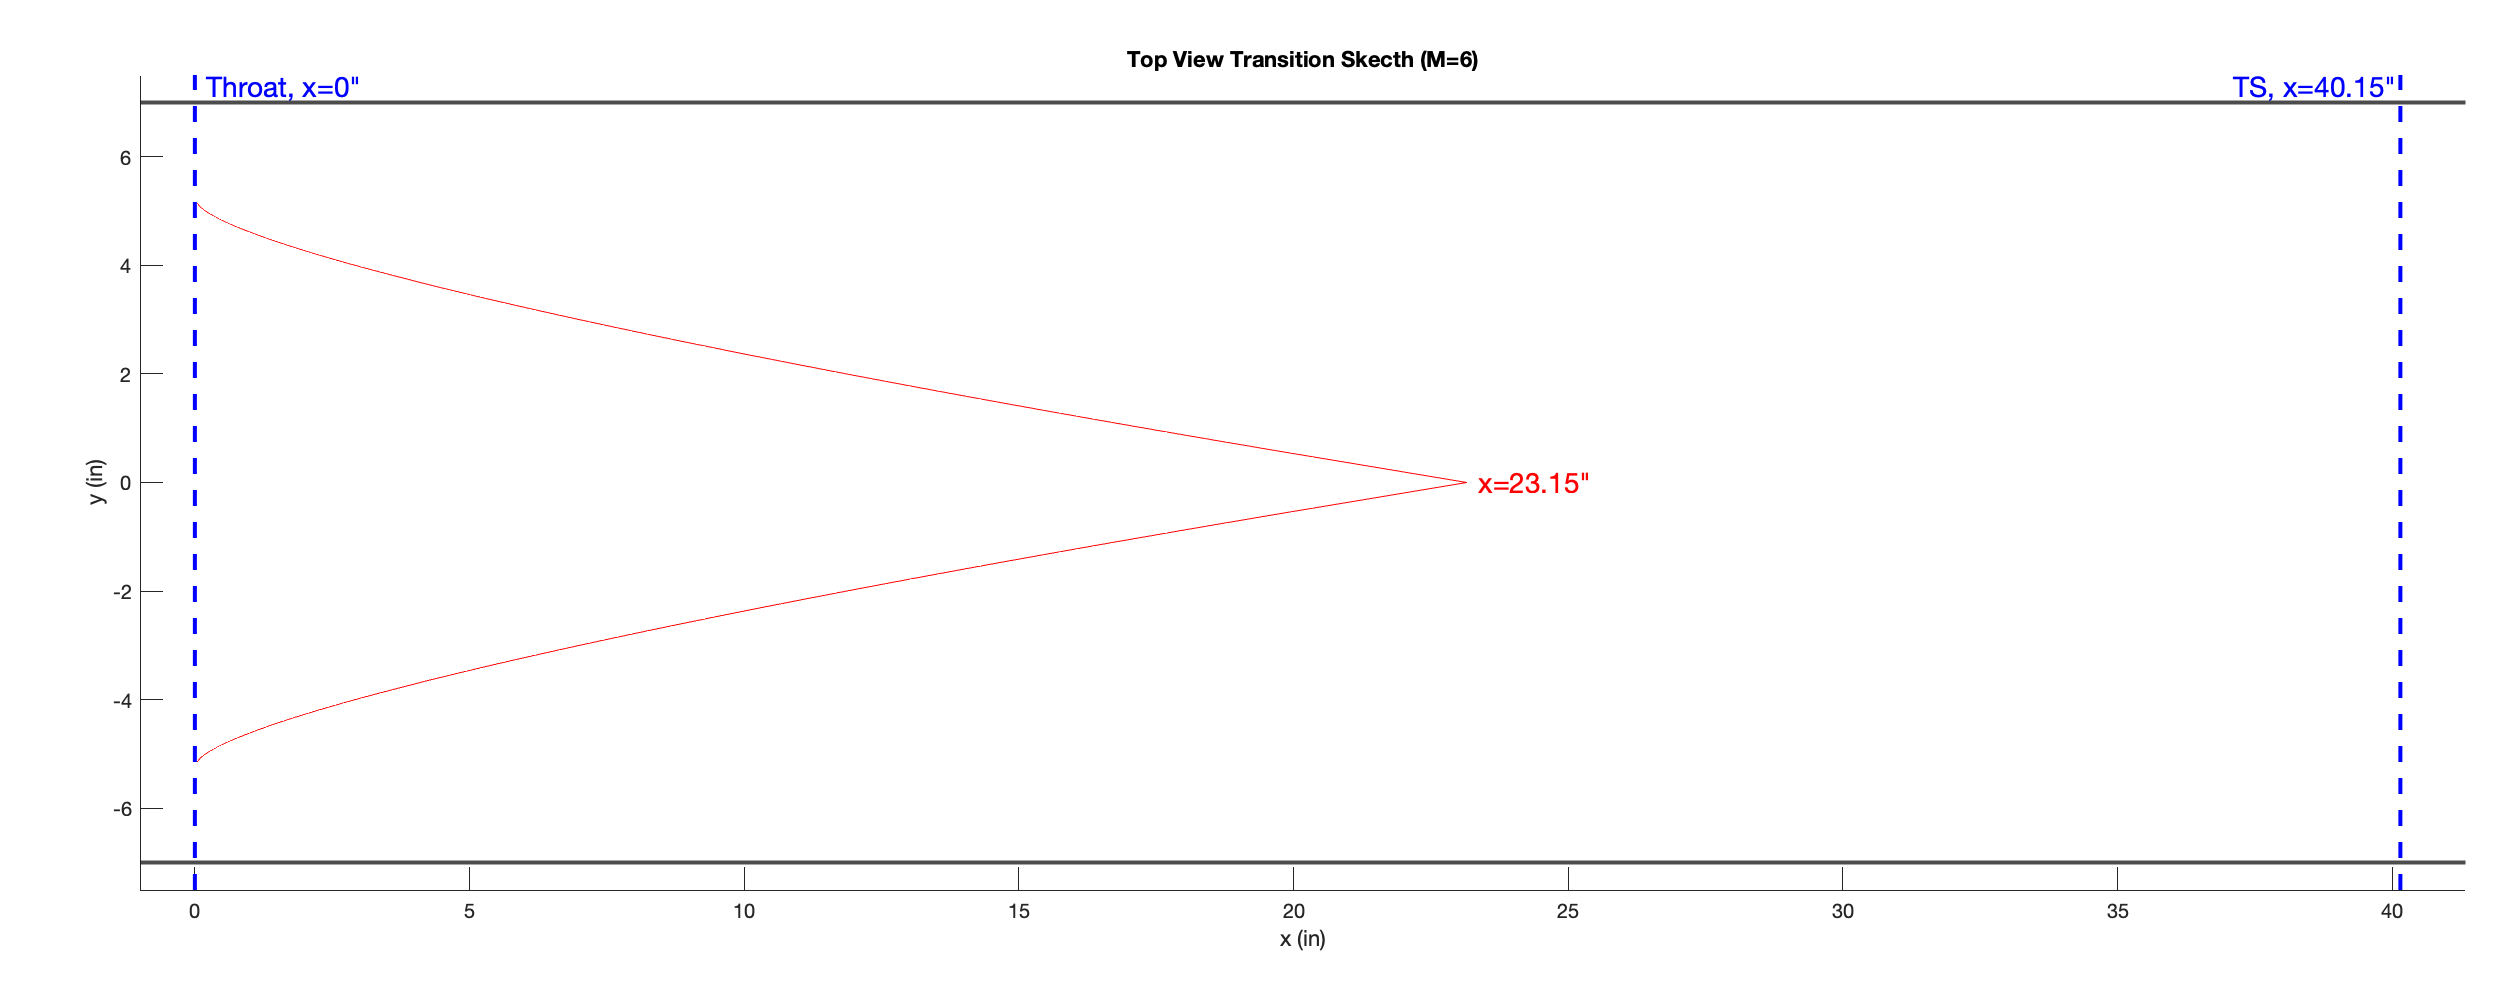
\includegraphics[width=6.5in]{top17}
    \caption{Mach lines for noise measured at 17" upstream on nozzle exit.}
    \label{fig:machlines}
\end{figure}

While both sidewall vortices and Görtler vortices can play some role in transition in planar nozzles, they are no longer considered suspects for the pressure fluctuation levels increase at unit Reynolds numbers above $3 \times 10^6/\mathrm{m}$.

\textcolor{red}{Rewrite. The combination of pitot surveys and characteristic tracing eliminates the possibility of sidewall mushroom vortices or Görtler vortices because these instabilities would lead to transition downstream of the characteristic wall origins found by tracing from the measurement location to the wall intersection. This leaves the surface discontinuity at the throat as the primary culprit for the pressure fluctuation levels increase. The remaining suspect mechanisms are still important to note and address in the redesign of the ACE tunnel.}

Following the above conclusions and recommendations, the most likely reason the pressure fluctuations increase is laminar-to-turbulent transition due to a surface discontinuity at the throat. This conclusion is supported by pitot surveys, CFD, and method of characteristics line tracing described above. 

\subsubsection*{Design Recommendations}

The following improvements are recommended to maintain laminar flow above $Re'$ $\approx 3 \times 10^6/\mathrm{m}$:
\begin{enumerate}
    \item Second-derivative-smooth subsonic-to-supersonic throat transition to eliminate nozzle throat discontinuity
    \item Continuous curvature with analytical functions to eliminate waviness and surface discontinuities
    \item Enhanced surface polishing to minimize surface roughness
    \item Improved settling chamber design to maximize flow uniformity and minimize freestream turbulence upstream of the nozzle throat
\end{enumerate}

\textcolor{red}{Paragraph about future possibility of subsonic boundary layer suction/bleed}

\section{ACE2.0 Design}

Following these recommendations, the nozzle will be redesigned and remanufactured to meet specific requirements that will ensure the best performance and potentially expand the laminar Reynolds number range. The decision to remanufacture the nozzle presents an opportunity to revise the nozzle and settling chamber design to achieve true active controllability, properly embodying the "ACE" name.

The rest of the chapter details the planned improvements to the ACE tunnel and specific design requirements that will achieve those improvements. In addition to a new nozzle, the settling chamber will also be redesigned to ensure the uniformity and reduce the turbulence of the flow into the nozzle. These improvements are to achieve the goal of increasing the unit Reynolds number at which laminar nozzle flow is maintained.

\subsection{Design Requirements}

ACE2.0 will maintain many characteristics while improving some, so many requirements are the same as the original ACE design. The new tunnel will still produce uniform Mach 5 to 8 flow in the 9 inches by 14 inches test section, withstand a total temperature of 530 K, and maintain a minimum engineering factor of safety (FOS) of 1.5 when operating at a total pressure of 200 psia.

\subsubsection*{Nozzle Requirements}

The current ACE nozzle successfully produces uniform Mach 5 to 8 flow in its core. In order to maintain this good performance and not introduce unknown parameters, the new nozzle will retain a very similar contour with slight improvements. The requirements that remain the same are that the nozzle must produce uniform flow for the entire Mach range, achieve maximum height deflection without exceeding a FOS of 1.5, and prevent leaks up to 200 psia.

The improvements to the nozzle and associated requirements will be a contour with continuous 1st and 2nd derivatives that is specified by analytical functions that will eliminate discontinuities and truncation error and a maximum allowable stress less than or equal to that found in the current ACE flexure at maximum deflection.

\subsubsection*{Settling Chamber Requirements}

The current ACE settling chamber design provides multiple opportunities to improve flow conditioning and ease of maintenance. The new settling chamber design will increase the length and height and allow for variable aerogrid/screen configurations. The requirements that remain the same are low freestream turbulence, thin stable wall boundary layers, maximum uniformity, and preventing leaks at a pressure of 200 psia. The implementation of these requirements will be improved in the new design to achieve improved incoming flow into the nozzle.

Following Reshotko et al. \cite{reshotko}, the length of the settling chamber shall accommodate a separation of 250 characteristic mesh sizes between screens allowing for adequate turbulence decay. The aerogrids will have a hexagonal perforation pattern to increase porosity and decrease pressure loss. The number of aerogrids and screens shall be variable to allow for future flow conditioning experiments. The inlet shall include a baffle system that will provide an acceptable initial distribution and mixing of the air received from the high-pressure inlet piping. The overall design will accommodate the option for future boundary layer suction slots.

A settling chamber height of 6 inches was chosen to keep the velocity as slow as possible without going below 10 ft/s for the majority of the Mach number range, according to Pope and Goin \cite{pope}. The reason for this minimum is to prevent thermal convection vortices from dominating the flow at the walls. The interior of ACE2.0 will also be heated prior to the start of the run to help avoid thermal gradients. 

% With this in mind, the height of 6 inches was chosen as a good compromise as seen in Table \ref{tab:sc_vel}.

% \begin{table}[ht!]
%     \centering
%     \begin{tabular}{|c|c|c|c|c|}
%         \cline{2-5}
%         \multicolumn{1}{c}{} & \multicolumn{4}{|c|}{\textbf{Mach Number}} \\ \hline
%         \textbf{Height} & 5 & 6 & 7 & 8 \\ \hline
%         4" & 73.57 & 34.55 & 17.64 & 9.66 \\ \hline
%         5" & 58.83 & 27.64 & 14.11 & 7.73 \\ \hline \hline
%         6" & 49.01 & 23.03 & 11.76 & 6.44 \\ \hline \hline
%         7" & 42.00 & 19.74 & 10.08 & 5.52 \\ \hline
%         8" & 36.75 & 17.27 & 8.82 & 4.83 \\ \hline
%         9" & 32.66 & 15.35 & 7.84 & 4.29 \\ \hline
%     \end{tabular}
%     \caption{Settling chamber velocities (ft/s) for combinations of settling chamber heights and Mach numbers.}
%     \label{tab:sc_vel}
% \end{table}
    
\subsection{Nozzle Contour Codes}

The multiple reflections method-of-characteristics (MOC) Fortran script written by Bowersox that produced the ACE nozzle contour was used for the new nozzle contour. In order to achieve continuous first and second derivative continuity, a section of the code was modified to produce a fourth-order expansion section instead of the original second-order curve. This allowed the expansion section to match the curvature of both the subsonic section and the straight section. The code modification is included in Appendix \ref{appendix:contour}, and a comparison of the original quadratic and the new quartic expansion sections is shown in Figure \ref{fig:throats}. In this figure, the ACE contour is directly from the MOC points and the ACE2.0 contour is specified by an analytic fourth-order polynomial. The waviness of the MOC points can be seen here, emphasizing the need to define the entire nozzle with analytic functions.

\begin{figure}[ht!]
    \centering
    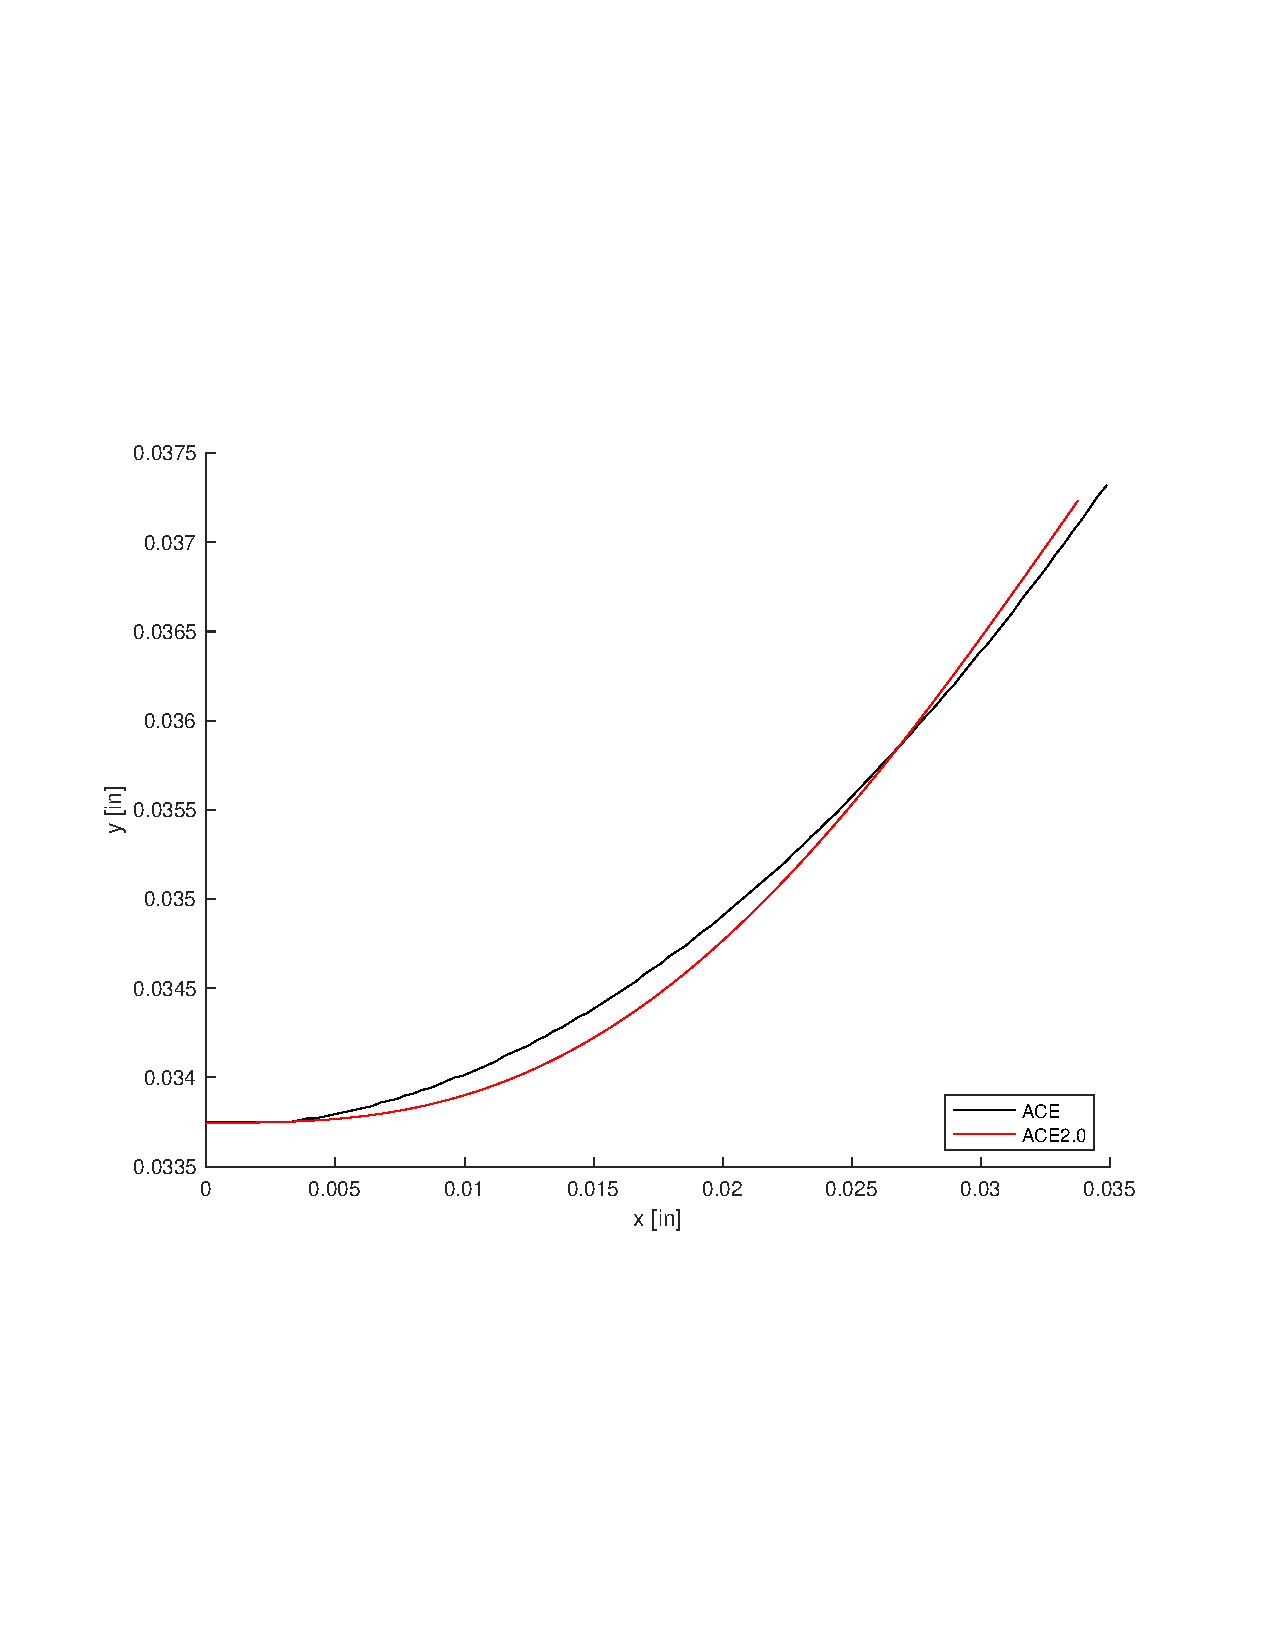
\includegraphics[trim={50 200 50 200},clip,width=6in]{throats.pdf}
    \caption{Comparison of ACE (quadratic) and ACE2.0 (quartic) expansion at throat}
    \label{fig:throats}
\end{figure}

After the MOC points were produced by the Fortran script, they were imported into a MATLAB script to fit with analytic functions. The subsonic curve is given by a fifth-order polynomial with six boundary conditions of $y(-L)=H$, $y'(-L)=0$, $y''(-L)=0$, $y(0)=h$, $y'(0)=0$, and $y''(0)=0$. \textcolor{red}{These condition require the nozzle contour...} The straightening section is given by a function found using the \texttt{lsqcurvefit} function with a combination of power and logarithmic functions in MATLAB. The equations for each section are given in Appendix \ref{appendix:contour}.

\subsection{CFD}

In order to verify the above nozzle contour performance compared to the original ACE contour, both contours were simulated in 2D CFD. First, a mesh was created in Pointwise for each contour with 400 equally spaced columns of cells in the x-direction. Each column had the spacing scaled to accurately capture the boundary layer with the smallest cell height around $4 \times 10^{-6}$ inches at the curved wall and the largest around 0.2 inches at the centerline as seen in Figure \ref{fig:mesh}. The CFD analysis was performed at a time when the settling chamber design was still at a height of 9 inches, so the analysis will be performed again to validate the 6 inch.

\begin{figure}[ht!]
    \centering
    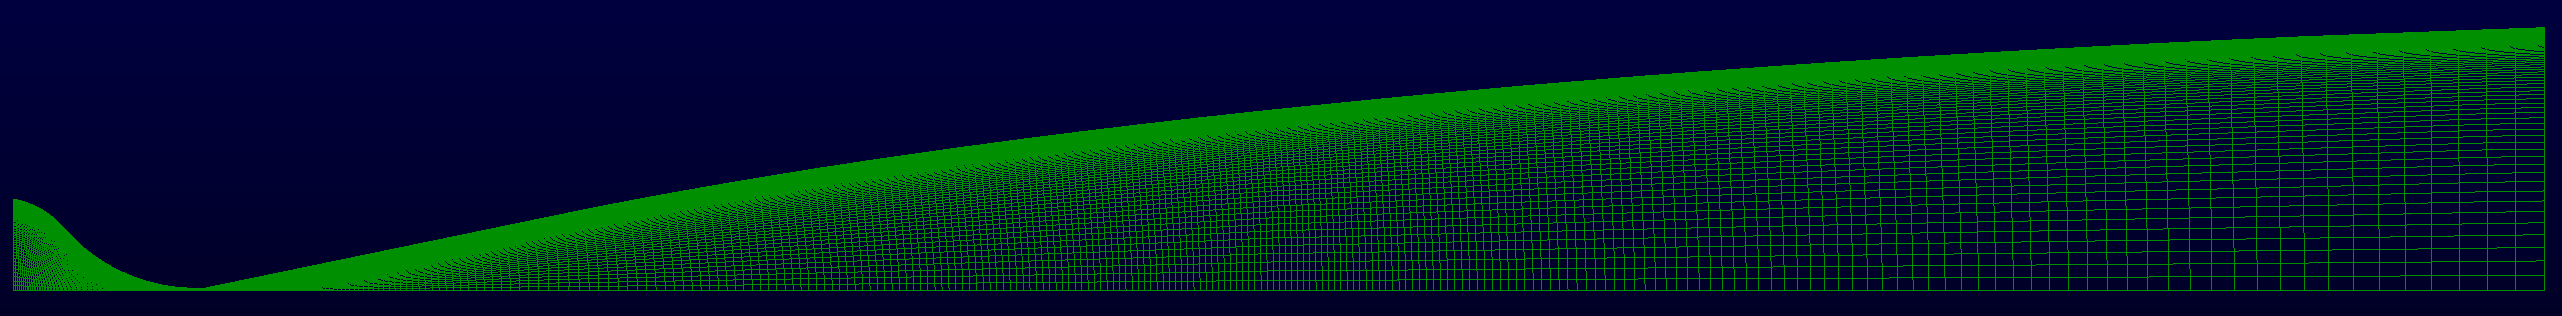
\includegraphics[width=6in]{ace-mesh}
    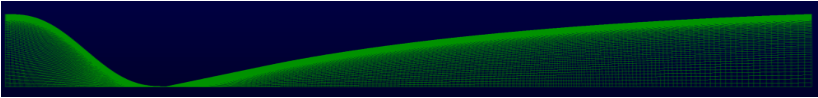
\includegraphics[width=6in]{qace-mesh}
    \caption{Mesh in Pointwise for ACE (top) and ACE2.0 (bottom) nozzle contours}
    \label{fig:mesh}
\end{figure}

After creating a mesh for each, they were simulated using US3D on the Texas A\&M supercomputer, Grace. \textcolor{red}{Stuff about inputs and convergence conditions followed by some results} 

A sample of the results is shown in Figure \ref{fig:ace2-cfd}. The full ACE2.0 CFD results compared to ACE is given in Appendix \ref{appendix:cfd}.

\begin{figure}[ht]
    \centering
    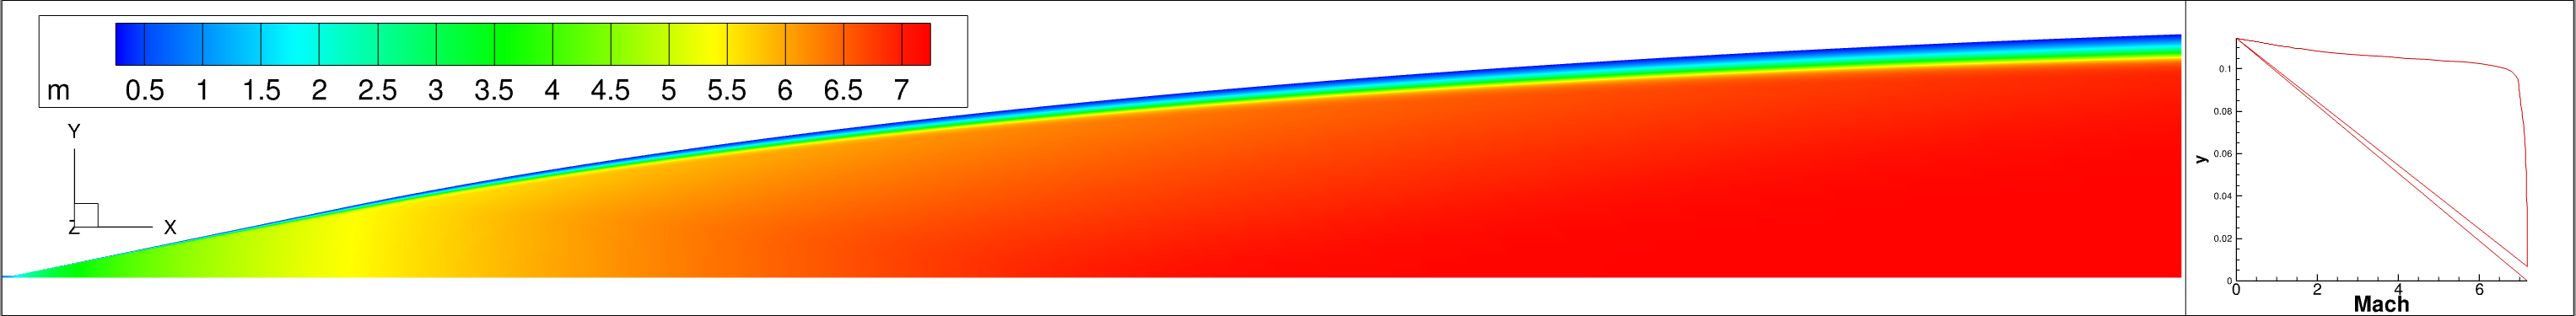
\includegraphics[width=6in]{ace2-cfd}
    \caption{ACE2.0 CFD Mach number plot}
    \label{fig:ace2-cfd}
\end{figure}

\subsection{Nozzle and Settling Chamber Design}

The resulting contour from above was imported into Solidworks using the analytic equations given in Appendix \ref{appendix:contour}, and the new ACE2.0 nozzle and settling chamber were designed following the above requirements. In order to accommodate the active control, the nozzle and settling chamber were combined into single rigid upper and lower pieces.Similar to ACE, the last 4 inches of the nozzle is a separate flexure piece to enable the variable Mach number capability. The overall length of the nozzle and settling chamber was increased by 19 inches with most of the added length contributed to the settling chamber. 

The settling chamber is 1.7 inches taller and has a few considerable improvements. The flow conditioners are enclosed in a standalone box that allows for easy maintenance and future modifications of screen configurations. The initial configuration provides 3 inches between each aerogrid and screen for adequate turbulence decay. Inlet flow spreaders are added as well to allow uniform mixing of the incoming air before flowing through the aerogrids. 

The ACE design had the relative motion interface between nozzle and settling chamber with a large rubber seal that struggled to properly seal at higher Mach numbers. For ACE2.0, the end of the settling chamber is split into two pieces to allow the rotation of the nozzle blocks. This moves the potential sealing issue upstream of the flow conditioners where minor leaks are much less of a concern. The final ACE2.0 nozzle and settling chamber design compared to ACE is shown in Figure \ref{fig:nozzles}. 

\begin{figure}[ht]
    \centering
    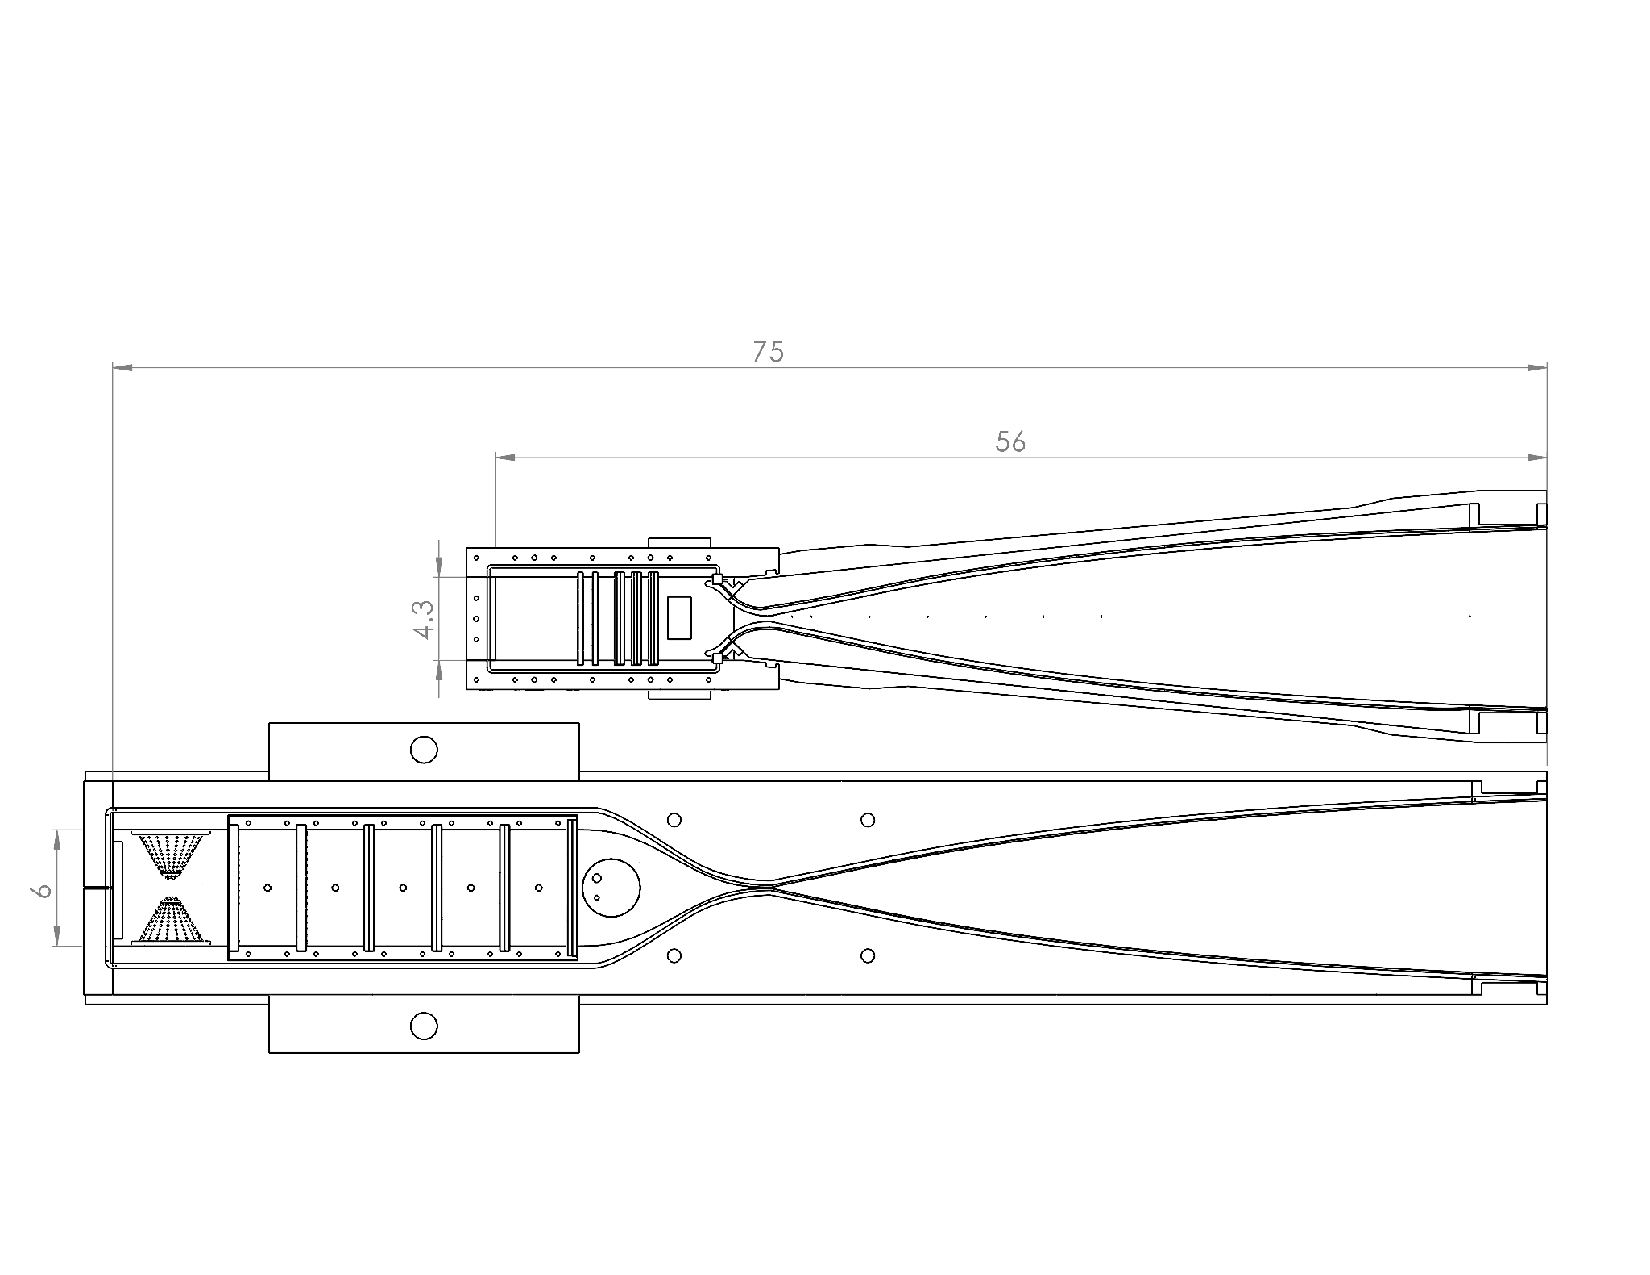
\includegraphics[trim={12 100 40 162},clip,width=6in]{nozzles.pdf}
    \caption{Comparison of ACE (top) and ACE2.0 (bottom) nozzle and settling chamber designs}
    \label{fig:nozzles}
\end{figure}

All of the nozzle and settling chamber parts will be made from 304 stainless steel except for the flexures, which will be made from Condition A 17-4 PH stainless steel for maximum strength while maintaining flexibility.

\subsection{Mechanical Design Iterations}

There were a few distinct iterations throughout the design process of ACE2.0 that are worth mentioning briefly. As mentioned, the original intent of the ACE redesign was not to enable active control, so the initial mechanical design was limited. 

\begin{figure}[ht]
    \centering
    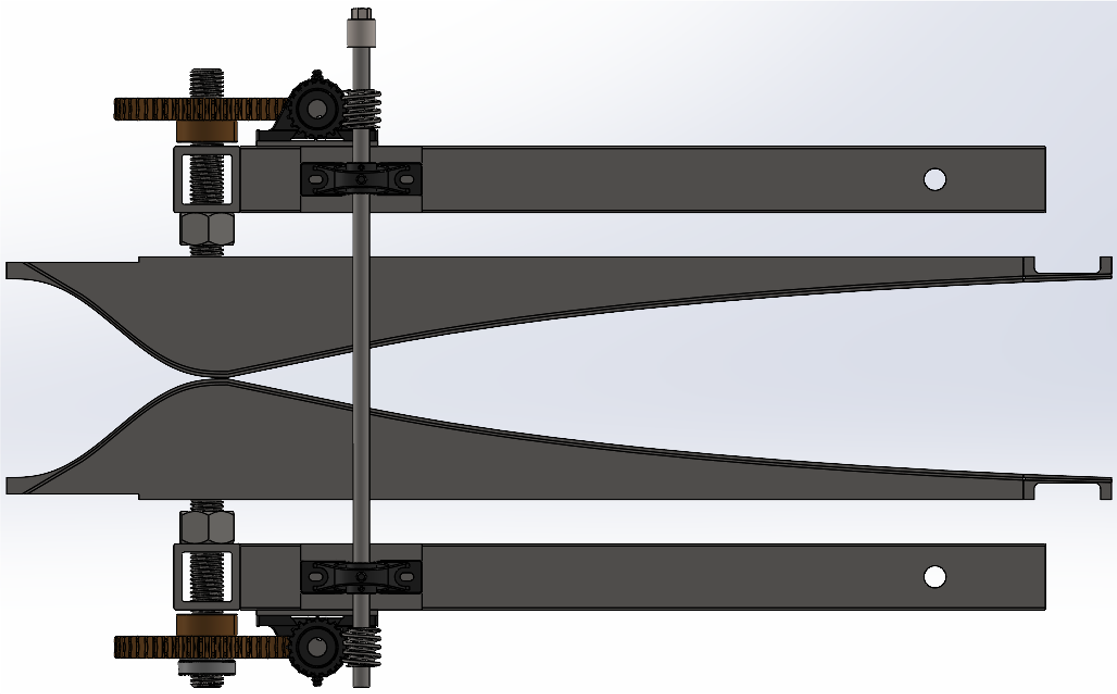
\includegraphics[width=5in]{i1a}
    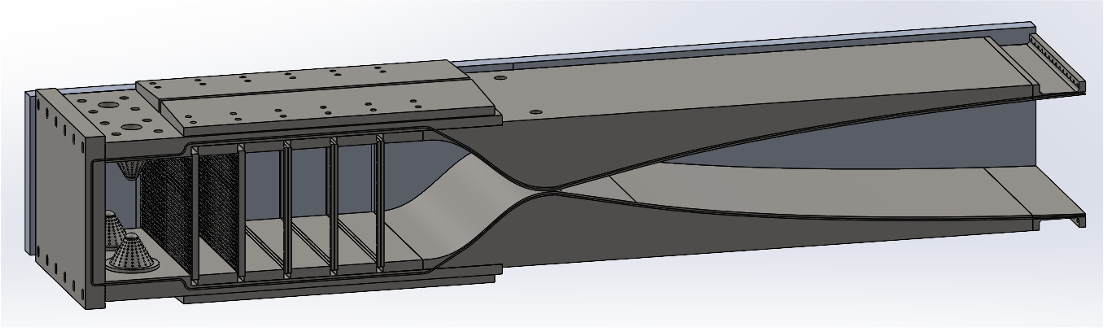
\includegraphics[width=5in]{i1b}
    \caption{Iteration 1 of ACE2.0: Non-active}
    \label{fig:i1}
\end{figure}

\begin{figure}[ht]
    \centering
    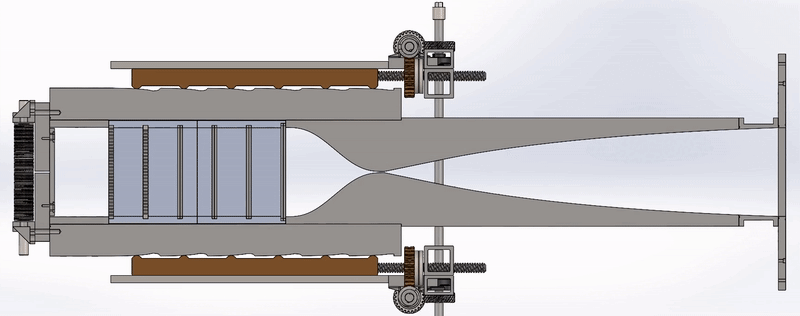
\includegraphics[width=6in]{i2}
    \caption{Iteration 2 of ACE2.0: Sliding Wedge}
    \label{fig:i2}
\end{figure}

\begin{figure}[ht]
    \centering
    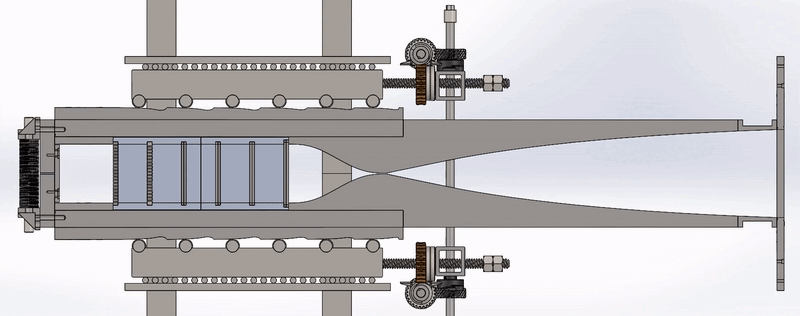
\includegraphics[width=6in]{i3}
    \caption{Iteration 3 of ACE2.0: Rollers}
    \label{fig:i3}
\end{figure}

\begin{figure}[ht]
    \centering
    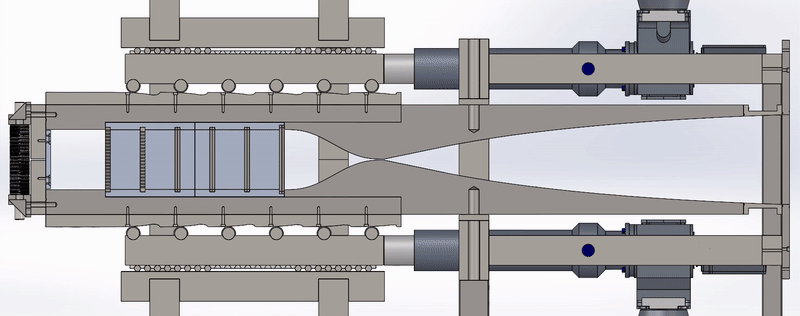
\includegraphics[width=6in]{i4}
    \caption{Iteration 4 of ACE2.0: Rollers and Actuators}
    \label{fig:i4}
\end{figure}

\subsection{20-Ton Linear Actuators Design}

The final iteration...

\subsubsection{Frame Design}

\textcolor{red}{Description and figures}

Originally planned to water jet bars from brace stock to save material cost and reduce excess. Later discovered that the cost of time and tooling on water jet to cut all pieces from 3 inch 4140 allot steel exceeds the cost of ordering bar stock.

\subsubsection{Actuation System Design}

\textcolor{red}{Detailed specifics of actuation components}

The actuation system will comprises 20-ton linear actuators, 20:1 gearboxes, servo motors, and a PLC to receive feedback inputs and control the system.

\subsubsection{Final Overall Design}

The entire design will integrate with the existing ACE test section and other infrastructure.

\textcolor{red}{Pictured below is the final overall ACE2.0 assembly.}

\begin{figure}[ht!]
    \centering
    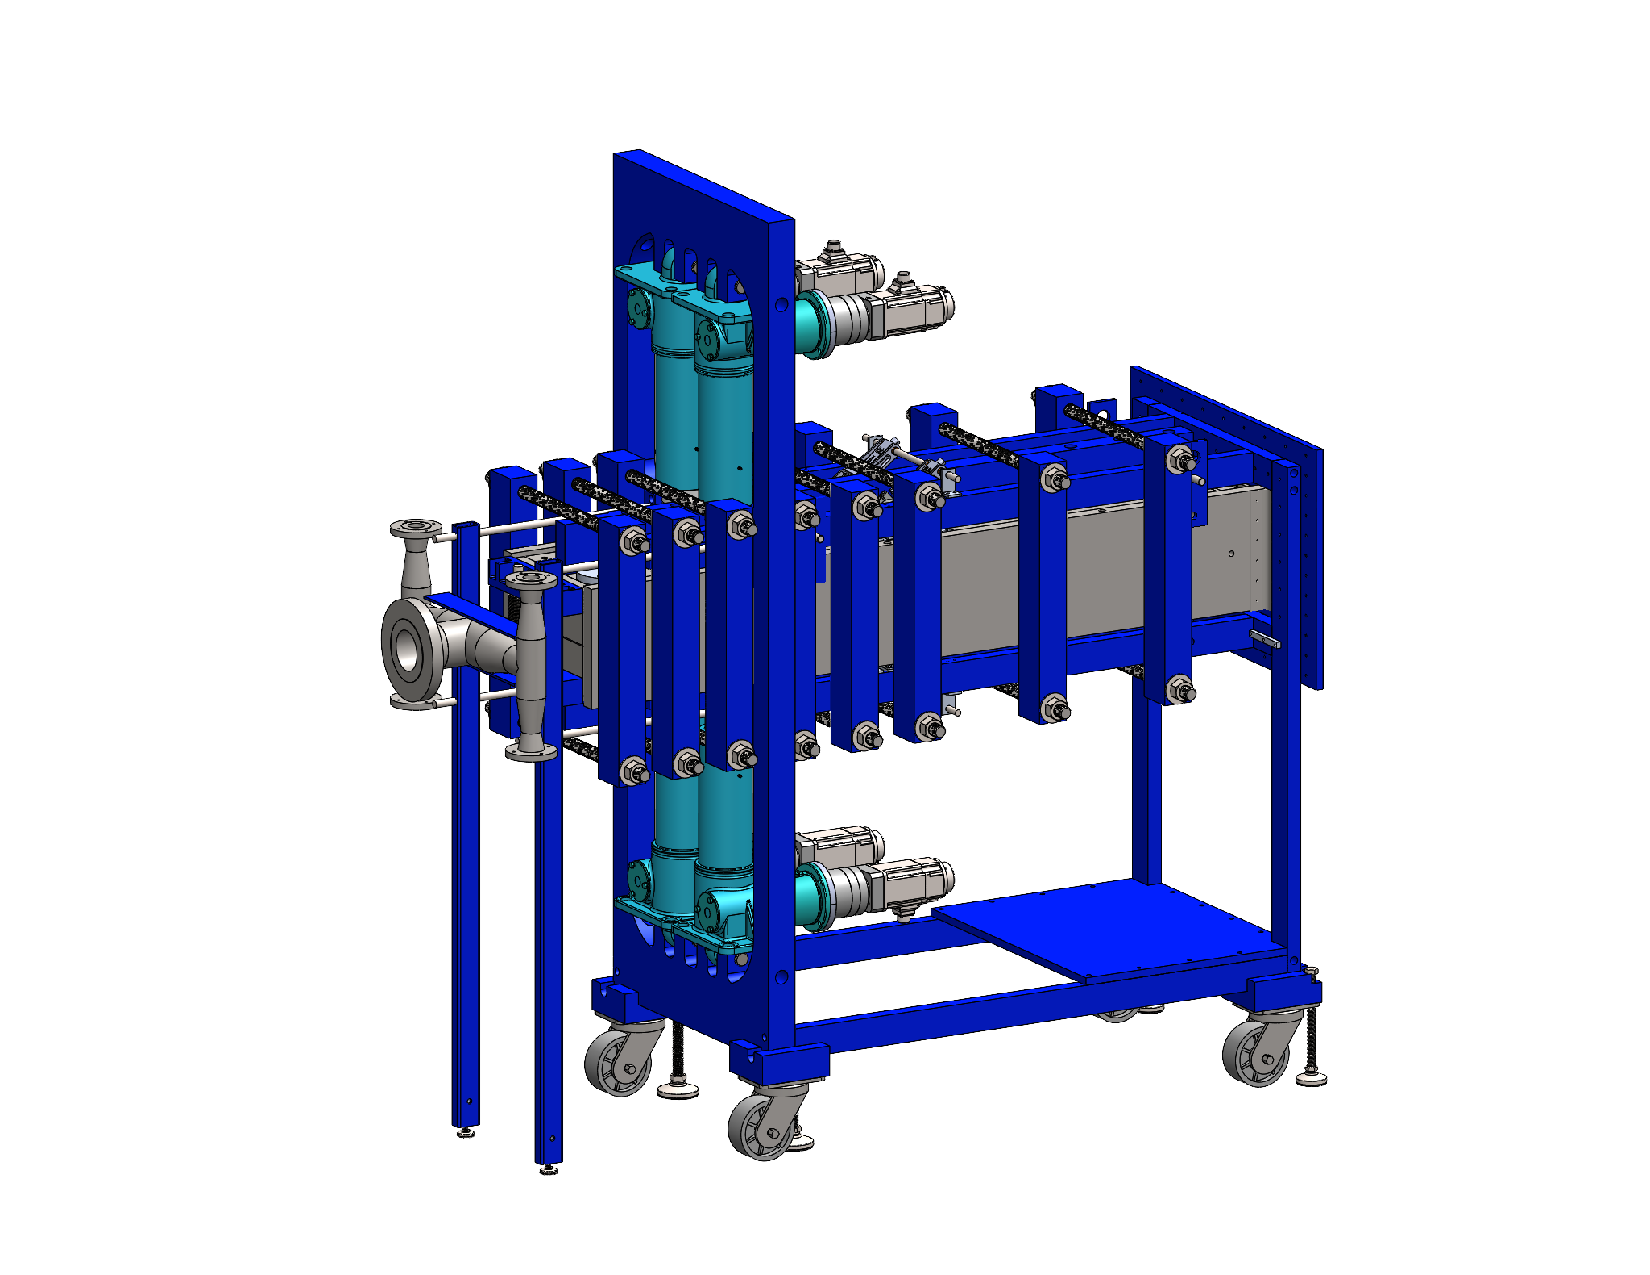
\includegraphics[width=6in]{cad-full}
    \caption{Temporary full CAD design}
    \label{fig:cad-full}
\end{figure}

\subsubsection{FEA}

\textcolor{red}{Stress and FOS stuff with figures}

\section{Fabrication Plans}

\textcolor{red}{How much to detail? Pictures of stock? What parts to show final machined?}

\textcolor{red}{ACE2.0 is currently being fabricated. Most machining is completed. Pictures of machining and fabrication.}

\begin{figure}[ht!]
    \centering
    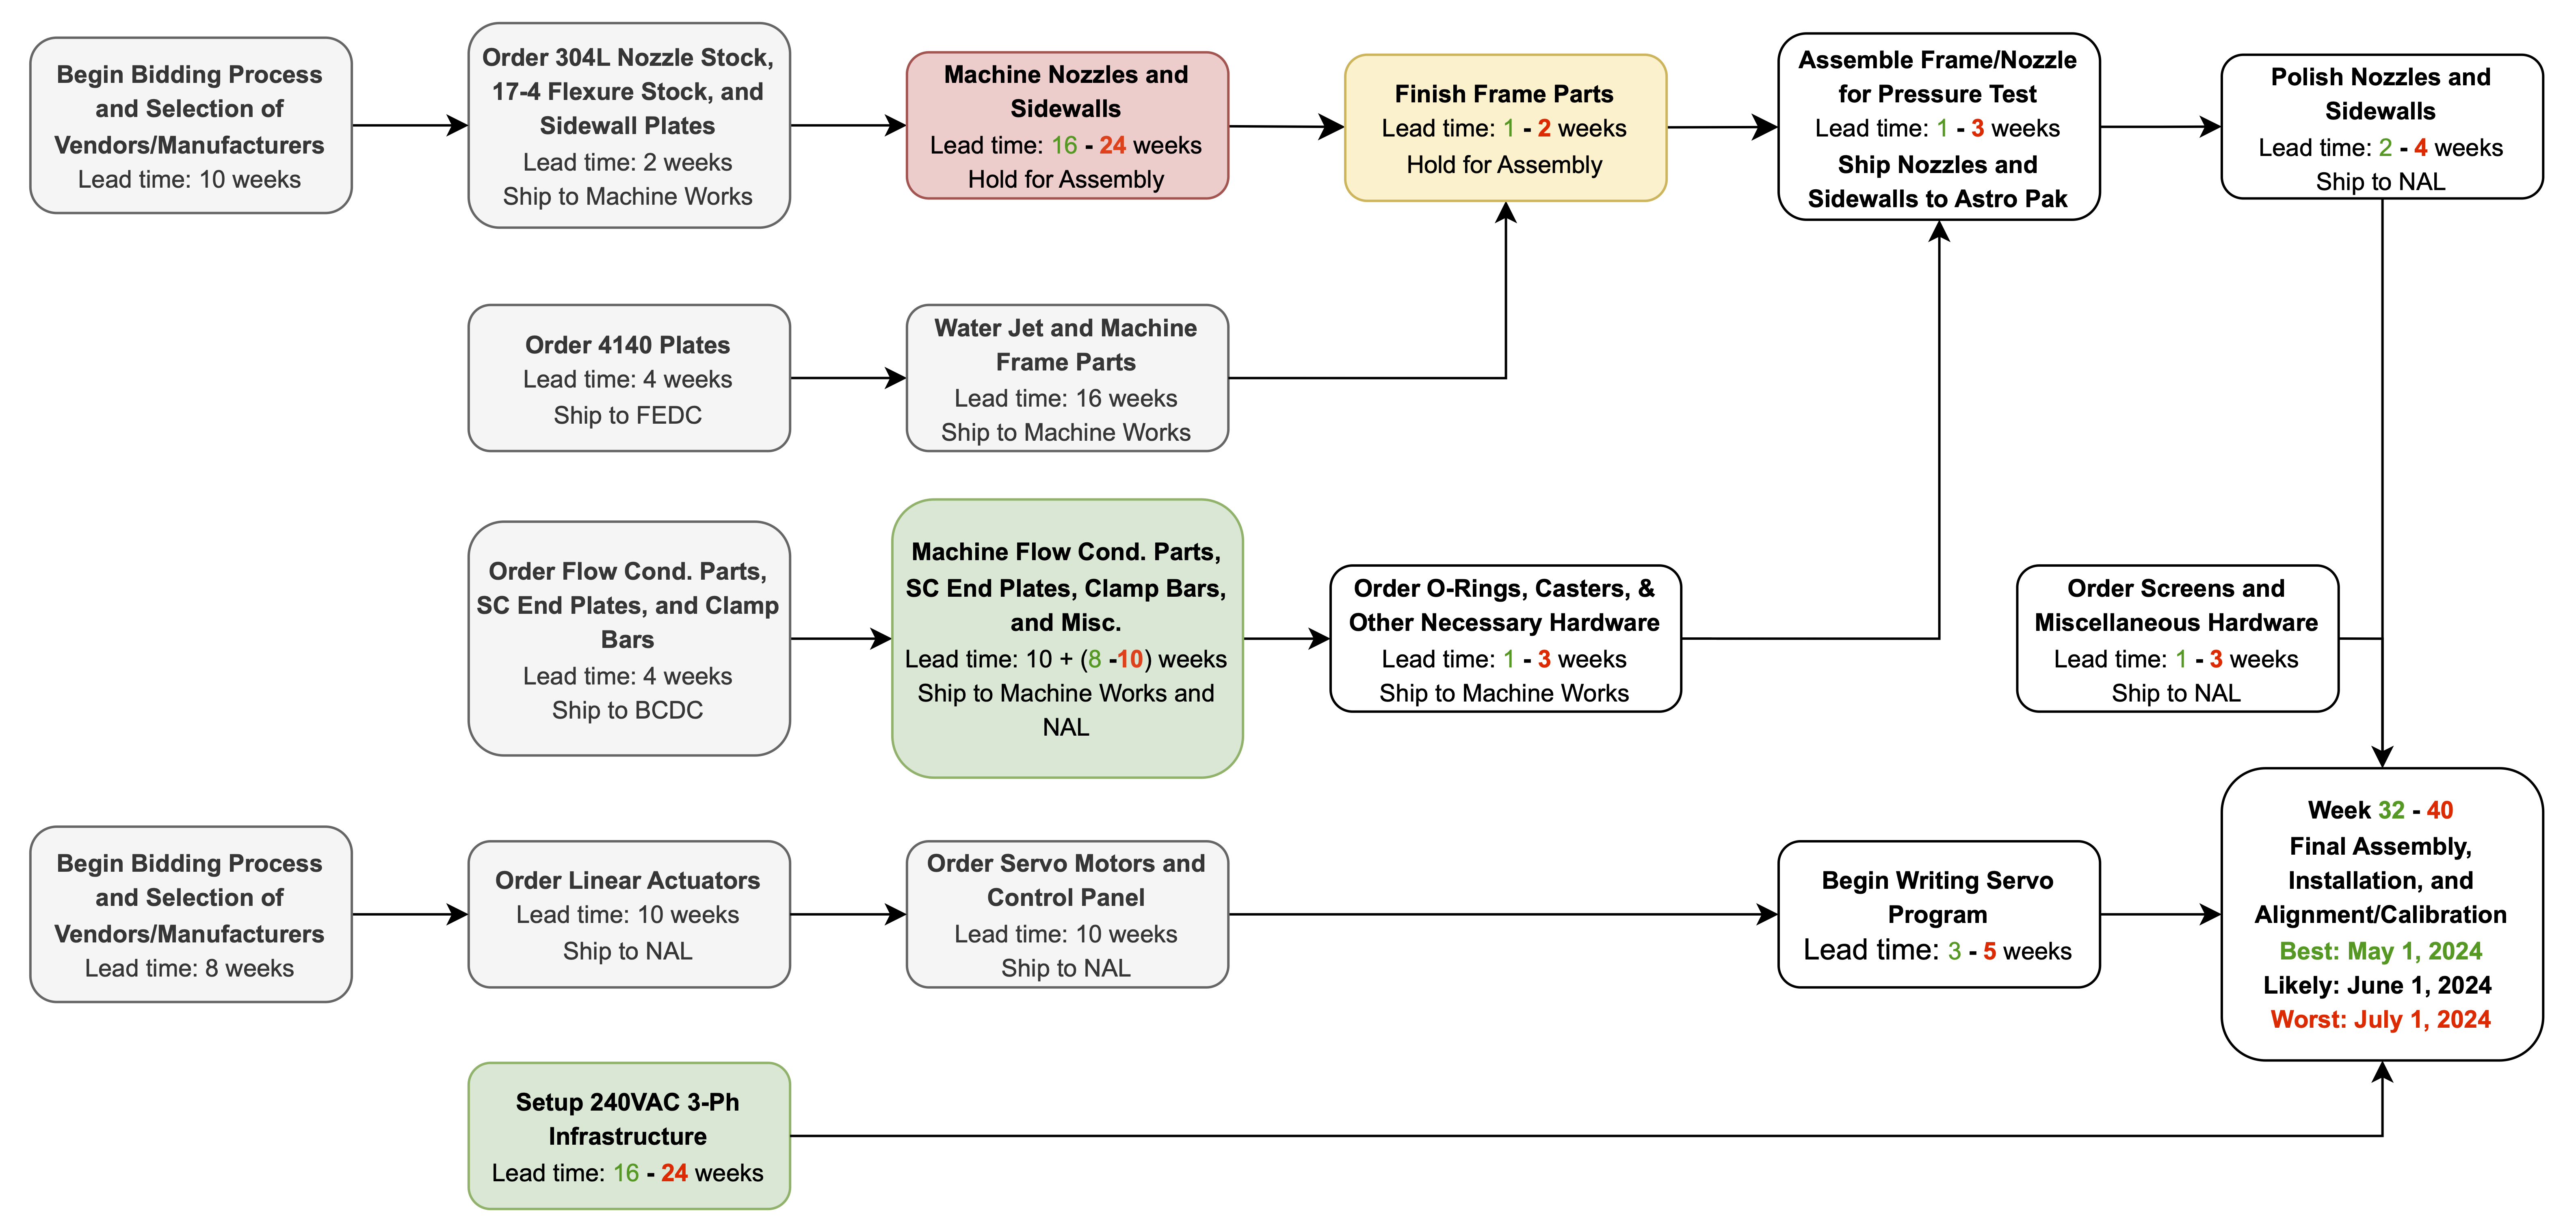
\includegraphics[width=6in]{schedule}
    \caption{Manufacturing schedule beginning from September 25, 2023.}
    \label{fig:schedule}
\end{figure}

\subsection{Pressure Test}

\textcolor{red}{Check structural integrity at 200 psia and evaluate sealing.}

\subsection{Polishing}

\textcolor{red}{Astro Pak polishing nozzles and sidewalls to 1 Ra.}

\section{Final Assembly, Installation, and Calibration}

The final assembly will occur at the NAHL. Once nozzles and actuators are assembled in the frame, ACE2.0 will be rolled into the lab to replace ACE. All hoses, wires, and instrumentation attached to the nozzle and settling chamber will be removed and ACE will be rolled out of the lab. ACE2.0 will roll in and reconnect all hoses, wires, and instrumentation.

\subsection{Actuation Homing and Calibration}

Before the sidewalls are installed, the nozzles will be aligned by homing the servo motors with the limit switches. At this point shims will be used to make fine adjustments to limit switch positions to ensure a minimum Mach number of \textcolor{red}{4.9} and a maximum Mach number of \textcolor{red}{8.5}.

\subsection{Shakedown and First Runs}

\textcolor{red}{Decide what the first runs' purposes should be to properly calibrate.}

